\documentclass[dvipdfmx]{jsarticle}
\setcounter{section}{5}
\setcounter{subsection}{3}
\usepackage{xr}
\externaldocument{4.5.2}
\externaldocument{4.5.3}
\usepackage{amsmath,amsfonts,amssymb,array,comment,mathtools,url,docmute}
\usepackage{longtable,booktabs,dcolumn,tabularx,mathtools,multirow,colortbl,xcolor}
\usepackage[dvipdfmx]{graphics}
\usepackage{bmpsize}
\usepackage{amsthm}
\usepackage{enumitem}
\setlistdepth{20}
\renewlist{itemize}{itemize}{20}
\setlist[itemize]{label=•}
\renewlist{enumerate}{enumerate}{20}
\setlist[enumerate]{label=\arabic*.}
\setcounter{MaxMatrixCols}{20}
\setcounter{tocdepth}{3}
\newcommand{\rotin}{\text{\rotatebox[origin=c]{90}{$\in $}}}
\newcommand{\amap}[6]{\text{\raisebox{-0.7cm}{\begin{tikzpicture} 
  \node (a) at (0, 1) {$\textstyle{#2}$};
  \node (b) at (#6, 1) {$\textstyle{#3}$};
  \node (c) at (0, 0) {$\textstyle{#4}$};
  \node (d) at (#6, 0) {$\textstyle{#5}$};
  \node (x) at (0, 0.5) {$\rotin $};
  \node (x) at (#6, 0.5) {$\rotin $};
  \draw[->] (a) to node[xshift=0pt, yshift=7pt] {$\textstyle{\scriptstyle{#1}}$} (b);
  \draw[|->] (c) to node[xshift=0pt, yshift=7pt] {$\textstyle{\scriptstyle{#1}}$} (d);
\end{tikzpicture}}}}
\newcommand{\twomaps}[9]{\text{\raisebox{-0.7cm}{\begin{tikzpicture} 
  \node (a) at (0, 1) {$\textstyle{#3}$};
  \node (b) at (#9, 1) {$\textstyle{#4}$};
  \node (c) at (#9+#9, 1) {$\textstyle{#5}$};
  \node (d) at (0, 0) {$\textstyle{#6}$};
  \node (e) at (#9, 0) {$\textstyle{#7}$};
  \node (f) at (#9+#9, 0) {$\textstyle{#8}$};
  \node (x) at (0, 0.5) {$\rotin $};
  \node (x) at (#9, 0.5) {$\rotin $};
  \node (x) at (#9+#9, 0.5) {$\rotin $};
  \draw[->] (a) to node[xshift=0pt, yshift=7pt] {$\textstyle{\scriptstyle{#1}}$} (b);
  \draw[|->] (d) to node[xshift=0pt, yshift=7pt] {$\textstyle{\scriptstyle{#2}}$} (e);
  \draw[->] (b) to node[xshift=0pt, yshift=7pt] {$\textstyle{\scriptstyle{#1}}$} (c);
  \draw[|->] (e) to node[xshift=0pt, yshift=7pt] {$\textstyle{\scriptstyle{#2}}$} (f);
\end{tikzpicture}}}}
\renewcommand{\thesection}{第\arabic{section}部}
\renewcommand{\thesubsection}{\arabic{section}.\arabic{subsection}}
\renewcommand{\thesubsubsection}{\arabic{section}.\arabic{subsection}.\arabic{subsubsection}}
\everymath{\displaystyle}
\allowdisplaybreaks[4]
\usepackage{vtable}
\theoremstyle{definition}
\newtheorem{thm}{定理}[subsection]
\newtheorem*{thm*}{定理}
\newtheorem{dfn}{定義}[subsection]
\newtheorem*{dfn*}{定義}
\newtheorem{axs}[dfn]{公理}
\newtheorem*{axs*}{公理}
\renewcommand{\headfont}{\bfseries}
\makeatletter
  \renewcommand{\section}{%
    \@startsection{section}{1}{\z@}%
    {\Cvs}{\Cvs}%
    {\normalfont\huge\headfont\raggedright}}
\makeatother
\makeatletter
  \renewcommand{\subsection}{%
    \@startsection{subsection}{2}{\z@}%
    {0.5\Cvs}{0.5\Cvs}%
    {\normalfont\LARGE\headfont\raggedright}}
\makeatother
\makeatletter
  \renewcommand{\subsubsection}{%
    \@startsection{subsubsection}{3}{\z@}%
    {0.4\Cvs}{0.4\Cvs}%
    {\normalfont\Large\headfont\raggedright}}
\makeatother
\makeatletter
\renewenvironment{proof}[1][\proofname]{\par
  \pushQED{\qed}%
  \normalfont \topsep6\p@\@plus6\p@\relax
  \trivlist
  \item\relax
  {
  #1\@addpunct{.}}\hspace\labelsep\ignorespaces
}{%
  \popQED\endtrivlist\@endpefalse
}
\makeatother
\renewcommand{\proofname}{\textbf{証明}}
\usepackage{tikz,graphics}
\usepackage[dvipdfmx]{hyperref}
\usepackage{pxjahyper}
\hypersetup{
 setpagesize=false,
 bookmarks=true,
 bookmarksdepth=tocdepth,
 bookmarksnumbered=true,
 colorlinks=false,
 pdftitle={},
 pdfsubject={},
 pdfauthor={},
 pdfkeywords={}}
\begin{document}
%\hypertarget{lebesgueux6e2cux5ea6}{%
\subsection{Lebesgue測度}%\label{lebesgueux6e2cux5ea6}}
%\hypertarget{ux6709ux9650ux52a0ux6cd5ux7684ux306alebesgue-stieltjesux6e2cux5ea6}{%
\subsubsection{有限加法的なLebesgue-Stieltjes測度}%\label{ux6709ux9650ux52a0ux6cd5ux7684ux306alebesgue-stieltjesux6e2cux5ea6}}
\begin{dfn}\label{区間}
$n$次元数空間$\mathbb{R}^{n}$において、$\forall i \in \varLambda_{n}$に対し、$- \infty \leq a_{i} \leq b_{i} \leq \infty$なる元々$a_{i}$、$b_{i}$を用いて次式のように書かれる集合$I$を$n$次元の区間ということにする。定義から分かるように、空集合もまた$n$次元の区間である。このような区間全体の集合を以下$\mathfrak{I}_{n}$と書くことにする。
\begin{align*}
I = \left\{ \mathbf{x} \in \mathbb{R}^{n} \middle| \mathbf{x} = \left( x_{i} \right)_{i \in \varLambda_{n}},\ \ \forall i \in \varLambda_{n}\left[ a_{i} < x_{i} \leq b_{i} \right] \right\} = \prod_{i \in \varLambda_{n}} \left( a_{i},b_{i} \right]
\end{align*}
\end{dfn}
\begin{dfn}\label{区間塊}
その集合$\mathfrak{I}_{n}$の互いに素な元の族$\left\{ I_{i} \right\}_{i \in \varLambda_{m} }$が与えられたとき、これの直和$\bigsqcup_{i \in \varLambda_{m} } I_{i}$を$n$次元の区間塊ということにする。定義から明らかに空集合もまた$n$次元の区間である。このような区間塊全体の集合を以下$\mathfrak{F}_{n}$と書くことにする。
\end{dfn}
\begin{dfn}\label{有限加法的なLebesgue-Stieltjes測度}
$\forall i \in \varLambda_{n}$に対し、関数$f_{i}:\mathbb{R} \rightarrow \mathbb{R}$が単調増加するようなその関数$F = \left( f_{i} \right)_{i \in \varLambda_{n}}:\mathbb{R} \rightarrow \mathbb{R}^{n}$が与えられたとき、次式のように写像$\psi_{F}:\mathfrak{I}_{n} \rightarrow \mathrm{cl}\mathbb{R}^{+}$が定義される。また、$\psi_{F}(\emptyset) = 0$と定義される。
\begin{align*}
\psi_{F}(I) = \sup\left\{ \prod_{i \in \varLambda_{n}} \left( f_{i}\left( b_{i}' \right) - f_{i}\left( a_{i}' \right) \right) \in \mathrm{cl}\mathbb{R}^{+} \middle| \forall\prod_{i \in \varLambda_{n}} \left( a_{i}',b_{i}' \right]\in \mathfrak{P}(I) \cap \mathfrak{I}_{n} \right\}
\end{align*}
さらに、次式のようにgraphが$G_{\varPsi_{F}}$の対応$\varPsi_{F}:\mathfrak{F}_{n} \multimap \mathrm{cl}\mathbb{R}^{+}$が定義される。
\begin{align*}
G_{\varPsi_{F}} = \left\{ (E,S) \in \mathfrak{F}_{n} \times \mathrm{cl}\mathbb{R}^{+} \middle| S = \sum_{i \in \varLambda_{m}} {\psi_{F}\left( I_{i} \right)},\ \ E = \bigsqcup_{i \in \varLambda_{m}} I_{i},\ \ \left\{ I_{i} \right\}_{i \in \varLambda_{m}} \subseteq \mathfrak{I}_{n} \right\}
\end{align*}
このような対応$\varPsi_{F}$は、実はのちに述べるように、写像どころかJordan測度をも成していることから、そのJordan測度$\varPsi_{F}:\mathfrak{F}_{n} \rightarrow \mathrm{cl}\mathbb{R}^{+}$を、ここでは、その関数$F:\mathbb{R} \rightarrow \mathbb{R}^{n}$についての有限加法的なLebesgue-Stieltjes測度ということにする\footnote{フランス人とオランダ人の人名なのでルベーグ、スティールティェスと読みます。フランス語って難しい…。}。
\end{dfn}\par
以下、$n$次元数空間$R^{n}$への拡張が容易であるかつ、記法的に煩雑になるため、簡単のため2次元数空間$\mathbb{R}^{2}$で考えることにしよう。
\begin{thm}\label{4.5.4.1} 上で定義された関数$F = \begin{pmatrix}
f \\
g \\
\end{pmatrix}:\mathbb{R} \rightarrow \mathbb{R}^{2}$についての写像$\psi_{F}:\mathfrak{I}_{2} \rightarrow \mathrm{cl}\mathbb{R}^{+}$について、$I = (a,b] \times (c,d]$なる区間$I$が有界な区間であるとき、次式が成り立つ。
\begin{align*}
\psi_{F}(I) = \left( f(b) - f(a) \right)\left( g(d) - g(c) \right)
\end{align*}\par
より一般に、上で定義された関数$F = \left( f_{i} \right)_{i \in \varLambda_{n}}:\mathbb{R} \rightarrow \mathbb{R}^{n}$についての写像$\psi_{F}:\mathfrak{I}_{n} \rightarrow \mathrm{cl}\mathbb{R}^{+}$について、$I = \prod_{i \in \varLambda_{n}} \left( a_{i},b_{i} \right]$なる区間$I$が有界な区間であるとき、次式が成り立つ。
\begin{align*}
\psi_{F}(I) = \prod_{i \in \varLambda_{n}} \left( f_{i}\left( b_{i} \right) - f_{i}\left( a_{i} \right) \right)
\end{align*}
\end{thm}
\begin{proof} 上で定義された関数$F = \begin{pmatrix}
f \\
g \\
\end{pmatrix}:\mathbb{R} \rightarrow \mathbb{R}^{2}$についての写像$\psi_{F}:\mathfrak{I}_{2} \rightarrow \mathrm{cl}\mathbb{R}^{+}$について、$I = (a,b] \times (c,d]$なる区間$I$が有界な区間であるなら、定義より$\alpha < a \leq b < \beta$、$\gamma < c \leq d < \delta$なる実数たち$\alpha$、$\beta$、$\gamma$、$\delta$が存在するので、$a,b,c,d \in \mathbb{R}$が成り立つ。ここで、$\forall\left( a',b' \right] \times \left( c',d' \right]\in \mathfrak{P}(I) \cap \mathfrak{I}_{2}$に対し、明らかに$a \leq a' \leq b' \leq b$、$c \leq c' \leq d' \leq d$が成り立つので、それらの関数たち$f$、$g$が単調増加することに注意すれば、やはり次式が成り立つ。
\begin{align*}
0 \leq f\left( b' \right) - f\left( a' \right) \leq f(b) - f(a),\ \ 0 \leq g\left( d' \right) - g\left( c' \right) \leq g(d) - g(c)
\end{align*}
したがって、次式が成り立つ。
\begin{align*}
0 \leq \left( f\left( b' \right) - f\left( a' \right) \right)\left( g\left( d' \right) - g\left( c' \right) \right) \leq \left( f(b) - f(a) \right)\left( g(d) - g(c) \right)
\end{align*}
以上より、次のようになる。
\begin{align*}
\psi_{F}(I) &= \sup\left\{ \left( f\left( b' \right) - f\left( a' \right) \right)\left( g\left( d' \right) - g\left( c' \right) \right) \in \mathrm{cl}\mathbb{R}^{+} \middle| \forall\left( a',b' \right] \times \left( c',d' \right]\in \mathfrak{P}(I) \cap \mathfrak{I}_{2} \right\}\\
&= \left( f(b) - f(a) \right)\left( g(d) - g(c) \right)
\end{align*}
\end{proof}
\begin{thm}\label{4.5.4.2}
$n$次元の区間全体の集合$\mathfrak{I}_{n}$に制限されたその対応$\varPsi_{F}|\mathfrak{I}_{n}$は上の写像$\psi_{F}$に等しくなる。
\end{thm}
\begin{proof}
$n$次元の区間全体の集合$\mathfrak{I}_{n}$に制限されたその対応$\varPsi_{F}|\mathfrak{I}_{n}$について、$\forall I \in \mathfrak{I}_{n}$に対し、元の族$\left\{ I \right\}$もやはりその集合$\mathfrak{I}_{n}$の元の族でもあるから、次式が成り立つ。
\begin{align*}
V\left( \varPsi_{F}|\left\{ I \right\} \right) = \left\{ \psi_{F}(I) \right\} = V\left( \psi_{F}|\left\{ I \right\} \right)
\end{align*}
よって、$\varPsi_{F}|\mathfrak{I}_{n} = \psi_{F}$が得られる。
\end{proof}
\begin{thm}\label{4.5.4.3}
$\forall E \in \mathfrak{F}_{2}$に対し、次式が成り立つかつ、互いに素なその集合$\mathfrak{I}_{2}$の元の族$\left\{ I_{i} \right\}_{i \in \varLambda_{n}}$が与えられたとき、
\begin{align*}
E = \bigsqcup_{i \in \varLambda_{n}} I_{i}
\end{align*}
上で定義された対応$\varPsi_{F}$によるその集合$E$の値はその族$\left\{ I_{i} \right\}_{i \in \varLambda_{n}}$によらなくその対応$\varPsi_{F}$は写像になる。\par
より一般に、$\forall E \in \mathfrak{F}_{n}$に対し、次式が成り立つかつ、互いに素なその集合$\mathfrak{I}_{n}$の元の族$\left\{ I_{i} \right\}_{i \in \varLambda_{m}}$が与えられたとき、
\begin{align*}
E = \bigsqcup_{i \in \varLambda_{m}} I_{i}
\end{align*}
上で定義された対応$\varPsi_{F}$によるその集合$E$の値はその族$\left\{ I_{i} \right\}_{i \in \varLambda_{m}}$によらなくその対応$\varPsi_{F}$は写像になる。
\end{thm}
\begin{proof}
$\forall E \in \mathfrak{F}_{2}$に対し、次式が成り立つかつ、互いに素なその集合$\mathfrak{I}_{2}$の2つの元の族々$\left\{ I_{i} \right\}_{i \in \varLambda_{m}}$、$\left\{ J_{j} \right\}_{j \in \varLambda_{n}}$が与えられたとき、
\begin{align*}
E = \bigsqcup_{i \in \varLambda_{m}} I_{i} = \bigsqcup_{j \in \varLambda_{n}} J_{j}
\end{align*}
\begin{center}
  \begin{tikzpicture}[auto]
    \draw[line width=0.5pt] (2.05,7)--(5,7);
    \draw[line width=0.5pt] (5,7)--(5,5.05);
    \draw[line width=0.5pt] (2.05,5)--(3,5);
    \draw[line width=0.5pt] (3,5)--(3,4.05);
    \draw[line width=0.5pt] (4.05,5)--(5,5);
    \draw[line width=0.5pt] (5,5)--(5,4.05);
    \draw[line width=0.5pt] (2.05,4)--(6,4);
    \draw[line width=0.5pt] (6,4)--(6,3.05);
    \draw[dashed] (2.05,7)--(2.05,5.05);
    \draw[dashed] (2.05,5.05)--(5,5.05);
    \draw[dashed] (2.05,5)--(2.05,4.05);
    \draw[dashed] (2.05,4.05)--(3,4.05);
    \draw[dashed] (4.05,5)--(4.05,4.05);
    \draw[dashed] (4.05,4.05)--(5,4.05);
    \draw[dashed] (2.05,4)--(2.05,3.05);
    \draw[dashed] (2.05,3.05)--(6,3.05);
    \draw[dotted] (2,3)--(2,2);
    \draw[dotted] (3,3)--(3,2);
    \draw[dotted] (4,3)--(4,2);
    \draw[dotted] (5,3)--(5,2);
    \draw[dotted] (6,3)--(6,2);
    \draw[dotted] (1,3)--(2,3);
    \draw[dotted] (1,4)--(2,4);
    \draw[dotted] (1,5)--(2,5);
    \draw[dotted] (1,7)--(2,7);
    \draw[->] (1,2)--(7,2);
    \draw[->] (1,2)--(1,8);
    \node (aa) at (3.5,6) {$I_1 $};
    \node (ab) at (2.5,4.5) {$I_2 $};
    \node (ac) at (4.5,4.5) {$I_3 $};
    \node (ad) at (4,3.5) {$I_4 $};
    \node (ba) at (2,1.5) {$a_1 $};
    \node (ba) at (2,1) {$a_2 $};
    \node (ba) at (2,0.5) {$a_4 $};
    \node (bb) at (3,1.5) {$a^2 $};
    \node (bc) at (4,1.5) {$a_3 $};
    \node (bd) at (5,1.5) {$a^1 $};
    \node (bd) at (5,1) {$a^3 $};
    \node (be) at (6,1.5) {$a^4 $};
    \node (ca) at (0.5,3) {$b_4 $};
    \node (cb) at (-0.5,4) {$b_2 $};
    \node (cb) at (0,4) {$b_3 $};
    \node (cb) at (0.5,4) {$b^4 $};
    \node (cc) at (-0.5,5) {$b_1 $};
    \node (cc) at (0,5) {$b^2 $};
    \node (cc) at (0.5,5) {$b^3 $};
    \node (cd) at (0.5,7) {$b^1 $};
    \draw[line width=0.5pt] (10.05,7)--(11,7);
    \draw[line width=0.5pt] (11,7)--(11,4.05);
    \draw[line width=0.5pt] (11.05,7)--(13,7);
    \draw[line width=0.5pt] (13,7)--(13,5.05);
    \draw[line width=0.5pt] (12.05,5)--(13,5);
    \draw[line width=0.5pt] (13,5)--(13,4.05);
    \draw[line width=0.5pt] (10.05,4)--(12,4);
    \draw[line width=0.5pt] (12,4)--(12,3.05);
    \draw[line width=0.5pt] (12.05,4)--(14,4);
    \draw[line width=0.5pt] (14,4)--(14,3.05);
    \draw[dashed] (10.05,7)--(10.05,4.05);
    \draw[dashed] (10.05,4.05)--(11,4.05);
    \draw[dashed] (11.05,7)--(11.05,5.05);
    \draw[dashed] (11.05,5.05)--(13,5.05);
    \draw[dashed] (12.05,5)--(12.05,4.05);
    \draw[dashed] (12.05,4.05)--(13,4.05);
    \draw[dashed] (10.05,4)--(10.05,3.05);
    \draw[dashed] (10.05,3.05)--(12,3.05);
    \draw[dashed] (12.05,4)--(12.05,3.05);
    \draw[dashed] (12.05,3.05)--(14,3.05);
    \draw[dotted] (10,3)--(10,2);
    \draw[dotted] (11,3)--(11,2);
    \draw[dotted] (12,3)--(12,2);
    \draw[dotted] (13,3)--(13,2);
    \draw[dotted] (14,3)--(14,2);
    \draw[dotted] (9,3)--(10,3);
    \draw[dotted] (9,4)--(10,4);
    \draw[dotted] (9,5)--(10,5);
    \draw[dotted] (9,7)--(10,7);
    \draw[->] (9,2)--(15,2);
    \draw[->] (9,2)--(9,8);
    \node (aa) at (10.5,5.5) {$J_1 $};
    \node (ab) at (12,6) {$J_2 $};
    \node (ac) at (12.5,4.5) {$J_3 $};
    \node (ad) at (11,3.5) {$J_4 $};
    \node (ae) at (13,3.5) {$J_5 $};
    \node (ba) at (10,1.5) {$c_1 $};
    \node (ba) at (10,1) {$c_4 $};
    \node (bb) at (11,1.5) {$c_2 $};
    \node (bb) at (11,1) {$c^1 $};
    \node (bc) at (12,1.5) {$c_3 $};
    \node (bc) at (12,1) {$c_5 $};
    \node (bc) at (12,0.5) {$c^4 $};
    \node (bd) at (13,1.5) {$c^2 $};
    \node (bd) at (13,1) {$c^3 $};
    \node (be) at (14,1.5) {$c^5 $};
    \node (ca) at (8,3) {$d_4 $};
    \node (ca) at (8.5,3) {$d_5 $};
    \node (cb) at (7,4) {$d_1 $};
    \node (cb) at (7.5,4) {$d_3 $};
    \node (cb) at (8,4) {$d^4 $};
    \node (cb) at (8.5,4) {$d^5 $};
    \node (cc) at (8,5) {$d_2 $};
    \node (cc) at (8.5,5) {$d^3 $};
    \node (cd) at (8,7) {$d^1 $};
    \node (cd) at (8.5,7) {$d^2 $};
  \end{tikzpicture}
\end{center}
$\forall i \in \varLambda_{m}$に対し、$I_{i} = \left( a_{i},a^{i} \right] \times \left( b_{i},b^{i} \right]$、$\forall j \in \varLambda_{n}$に対し、$J_{j} = \left( c_{j},c^{j} \right] \times \left( d_{j},d^{j} \right]$とおき、$\forall i \in \varLambda_{m}\forall j \in \varLambda_{n}$に対し、元々$a_{i}$、$a^{i}$、$c_{j}$、$c^{j}$のうち相異なるもの全体を小さい順から並べたものを$\alpha_{1}$、$\alpha_{2}$、$\cdots$、$\alpha_{M}$、$\forall i \in \varLambda_{m}\forall j \in \varLambda_{n}$に対し、元々$b_{i}$、$b^{i}$、$d_{j}$、$d^{j}$のうち相異なるもの全体を小さい順から並べたものを$\beta_{1}$、$\beta_{2}$、$\cdots$、$\beta_{N}$とおき、
\begin{center}
  \begin{tikzpicture}[auto]
    \draw[line width=0.5pt] (2.05,6)--(5,6);
    \draw[line width=0.5pt] (5,6)--(5,3);
    %\draw[line width=0.5pt] (2.05,4)--(3,4);
    \draw[line width=0.5pt] (3,4.05)--(3,3);
    \draw[line width=0.5pt] (5,3)--(6,3);
    %\draw[line width=0.5pt] (5,4)--(5,3.05);
    \draw[line width=0.5pt] (3,3)--(4.05,3);
    \draw[line width=0.5pt] (6,3)--(6,2.05);
    \draw[dashed] (2.05,6)--(2.05,2.05);
    \draw[dashed] (3,4.05)--(4.05,4.05);
    %\draw[dashed] (2.05,4)--(2.05,3.05);
    %\draw[dashed] (2.05,3.05)--(3,3.05);
    \draw[dashed] (4.05,4.05)--(4.05,3);
    %\draw[dashed] (4.05,3.05)--(5,3.05);
    %\draw[dashed] (2.05,3)--(2.05,2.05);
    \draw[dashed] (2.05,2.05)--(6,2.05);
    \draw[dotted] (2,2)--(2,1);
    \draw[dotted] (3,2)--(3,1);
    \draw[dotted] (4,2)--(4,1);
    \draw[dotted] (5,2)--(5,1);
    \draw[dotted] (6,2)--(6,1);
    \draw[dotted] (1,2)--(2,2);
    \draw[dotted] (1,3)--(2,3);
    \draw[dotted] (1,4)--(2,4);
    \draw[dotted] (1,6)--(2,6);
    \draw[->] (1,1)--(7,1);
    \draw[->] (1,1)--(1,7);
    \node (aa) at (3.5,5) {$E $};
    \node (ba) at (2,0.5) {$\alpha_1 $};
    \node (bb) at (3,0.5) {$\alpha_2 $};
    \node (bc) at (4,0.5) {$\alpha_3 $};
    \node (bd) at (5,0.5) {$\alpha_4 $};
    \node (be) at (6,0.5) {$\alpha_5 $};
    \node (ca) at (0.5,2) {$\beta_1 $};
    \node (cb) at (0.5,3) {$\beta_2 $};
    \node (cc) at (0.5,4) {$\beta_3 $};
    \node (cd) at (0.5,6) {$\beta_4 $};
  \end{tikzpicture}
\end{center}
$\forall k \in \varLambda_{M - 1}\forall l \in \varLambda_{N - 1}$に対し、次式のように定義される区間$K(k,l)$を考えよう。このような区間全体の集合を$\mathfrak{K}$とおく。
\begin{align*}
K(k,l) = \left( \alpha_{k},\alpha_{k + 1} \right] \times \left( \beta_{l},\beta_{l + 1} \right]
\end{align*}
\begin{center}
  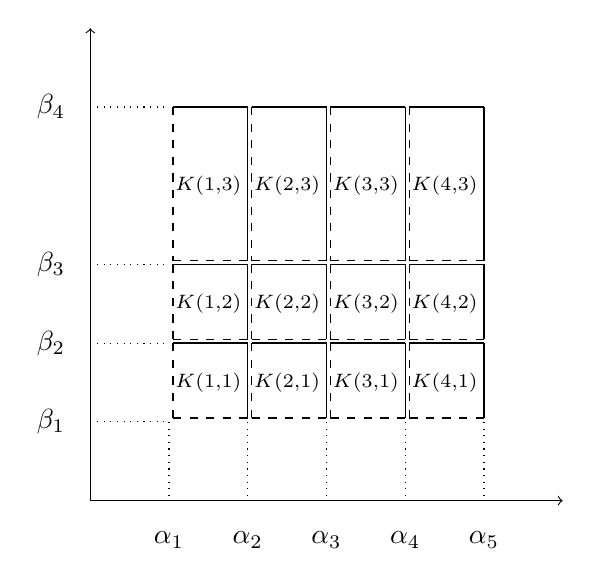
\begin{tikzpicture}[auto]
    \draw[line width=0.5pt] (2.05,3)--(3,3);
    \draw[line width=0.5pt] (3,3)--(3,2.05);
    \draw[line width=0.5pt] (3.05,3)--(4,3);
    \draw[line width=0.5pt] (4,3)--(4,2.05);
    \draw[line width=0.5pt] (4.05,3)--(5,3);
    \draw[line width=0.5pt] (5,3)--(5,2.05);
    \draw[line width=0.5pt] (5.05,3)--(6,3);
    \draw[line width=0.5pt] (6,3)--(6,2.05);
    \draw[line width=0.5pt] (2.05,4)--(3,4);
    \draw[line width=0.5pt] (3,4)--(3,3.05);
    \draw[line width=0.5pt] (3.05,4)--(4,4);
    \draw[line width=0.5pt] (4,4)--(4,3.05);
    \draw[line width=0.5pt] (4.05,4)--(5,4);
    \draw[line width=0.5pt] (5,4)--(5,3.05);
    \draw[line width=0.5pt] (5.05,4)--(6,4);
    \draw[line width=0.5pt] (6,4)--(6,3.05);
    \draw[line width=0.5pt] (2.05,6)--(3,6);
    \draw[line width=0.5pt] (3,6)--(3,4.05);
    \draw[line width=0.5pt] (3.05,6)--(4,6);
    \draw[line width=0.5pt] (4,6)--(4,4.05);
    \draw[line width=0.5pt] (4.05,6)--(5,6);
    \draw[line width=0.5pt] (5,6)--(5,4.05);
    \draw[line width=0.5pt] (5.05,6)--(6,6);
    \draw[line width=0.5pt] (6,6)--(6,4.05);
    \draw[dashed] (2.05,3)--(2.05,2.05);
    \draw[dashed] (2.05,2.05)--(3,2.05);
    \draw[dashed] (3.05,3)--(3.05,2.05);
    \draw[dashed] (3.05,2.05)--(4,2.05);
    \draw[dashed] (4.05,3)--(4.05,2.05);
    \draw[dashed] (4.05,2.05)--(5,2.05);
    \draw[dashed] (5.05,3)--(5.05,2.05);
    \draw[dashed] (5.05,2.05)--(6,2.05);
    \draw[dashed] (2.05,4)--(2.05,3.05);
    \draw[dashed] (2.05,3.05)--(3,3.05);
    \draw[dashed] (3.05,4)--(3.05,3.05);
    \draw[dashed] (3.05,3.05)--(4,3.05);
    \draw[dashed] (4.05,4)--(4.05,3.05);
    \draw[dashed] (4.05,3.05)--(5,3.05);
    \draw[dashed] (5.05,4)--(5.05,3.05);
    \draw[dashed] (5.05,3.05)--(6,3.05);
    \draw[dashed] (2.05,6)--(2.05,4.05);
    \draw[dashed] (2.05,4.05)--(3,4.05);
    \draw[dashed] (3.05,6)--(3.05,4.05);
    \draw[dashed] (3.05,4.05)--(4,4.05);
    \draw[dashed] (4.05,6)--(4.05,4.05);
    \draw[dashed] (4.05,4.05)--(5,4.05);
    \draw[dashed] (5.05,6)--(5.05,4.05);
    \draw[dashed] (5.05,4.05)--(6,4.05);
    \draw[dotted] (2,2)--(2,1);
    \draw[dotted] (3,2)--(3,1);
    \draw[dotted] (4,2)--(4,1);
    \draw[dotted] (5,2)--(5,1);
    \draw[dotted] (6,2)--(6,1);
    \draw[dotted] (1,2)--(2,2);
    \draw[dotted] (1,3)--(2,3);
    \draw[dotted] (1,4)--(2,4);
    \draw[dotted] (1,6)--(2,6);
    \draw[->] (1,1)--(7,1);
    \draw[->] (1,1)--(1,7);
    \node (aaa) at (2.5,2.5) {$\scriptstyle K\left( 1,1\right) $};
    \node (aab) at (3.5,2.5) {$\scriptstyle K\left( 2,1\right) $};
    \node (aac) at (4.5,2.5) {$\scriptstyle K\left( 3,1\right) $};
    \node (aad) at (5.5,2.5) {$\scriptstyle K\left( 4,1\right) $};
    \node (aba) at (2.5,3.5) {$\scriptstyle K\left( 1,2\right) $};
    \node (abb) at (3.5,3.5) {$\scriptstyle K\left( 2,2\right) $};
    \node (abc) at (4.5,3.5) {$\scriptstyle K\left( 3,2\right) $};
    \node (abd) at (5.5,3.5) {$\scriptstyle K\left( 4,2\right) $};
    \node (aca) at (2.5,5) {$\scriptstyle K\left( 1,3\right) $};
    \node (acb) at (3.5,5) {$\scriptstyle K\left( 2,3\right) $};
    \node (acc) at (4.5,5) {$\scriptstyle K\left( 3,3\right) $};
    \node (acd) at (5.5,5) {$\scriptstyle K\left( 4,3\right) $};
    \node (ba) at (2,0.5) {$\alpha_1 $};
    \node (bb) at (3,0.5) {$\alpha_2 $};
    \node (bc) at (4,0.5) {$\alpha_3 $};
    \node (bd) at (5,0.5) {$\alpha_4 $};
    \node (be) at (6,0.5) {$\alpha_5 $};
    \node (ca) at (0.5,2) {$\beta_1 $};
    \node (cb) at (0.5,3) {$\beta_2 $};
    \node (cc) at (0.5,4) {$\beta_3 $};
    \node (cd) at (0.5,6) {$\beta_4 $};
  \end{tikzpicture}
\end{center}
このとき、その集合$\mathfrak{K}$の全ての元々が互いに素であるから、次式を満たすようなその集合$\mathfrak{K}$の元の族$\left\{ K_{i} \right\}_{i \in \varLambda_{p}}$が存在する。
\begin{align*}
E = \bigsqcup_{i \in \varLambda_{p}} K_{i}
\end{align*}
ここで、その集合$\mathfrak{K}$の濃度$\#\mathfrak{K}$が数学的帰納法により明らかに$(M - 1)(N - 1)$に等しくこれはその集合$E$を覆うような長方形を考えたとき、この長方形がその集合$\mathfrak{K}$の直和として表されることに注意すれば、その集合はその長方形に等しいかその長方形から一部のその集合$\mathfrak{K}$の元々が欠けているような集合であるから、$p \leq (M - 1)(N - 1)$が成り立つ。さらに、その集合$\mathfrak{K}$の各元は元々$\alpha_{1}$、$\alpha_{2}$、$\cdots$、$\alpha_{M}$、$\beta_{1}$、$\beta_{2}$、$\cdots$、$\beta_{N}$の定義よりどれか1つの区間$I_{i}$に含まれているので、次式を満たすようなその集合$\mathfrak{K}$の元の族$\left\{ K_{ij} \right\}_{j \in \varLambda_{k_{i}}}$を考えれば、
\begin{align*}
I_{i} = \bigsqcup_{j \in \varLambda_{k_{i}}} K_{ij}
\end{align*}
その元の族$\left\{ K_{ij} \right\}_{j \in \varLambda_{k_{i}}}$もまたその集合$\mathfrak{I}_{2}$の部分集合で$I_{i} \in \mathfrak{F}_{2}$が成り立つので、その写像$\varPsi_{F}$を用いれば、やはり次式が成り立つことから、
\begin{align*}
\psi_{F}\left( I_{i} \right) = \varPsi_{F}\left( I_{i} \right) = \varPsi_{F}\left( \bigsqcup_{j \in \varLambda_{k_{i}}} K_{ij} \right) = \sum_{j \in \varLambda_{k_{i}}} {\psi_{F}\left( K_{ij} \right)}
\end{align*}
したがって、次式が成り立つので、
\begin{align*}
\sum_{i \in \varLambda_{m}} {\psi_{F}\left( I_{i} \right)} = \sum_{i \in \varLambda_{m}} {\sum_{j \in \varLambda_{k_{i}}} {\psi_{F}\left( K_{ij} \right)}}
\end{align*}
添数の付け替えにより次式が成り立つことに注意すれば、
\begin{align*}
\sum_{i \in \varLambda_{m}} {\sum_{j \in \varLambda_{k_{i}}} {\psi_{F}\left( K_{ij} \right)}} = \sum_{i \in \varLambda_{p}} {\psi_{F}\left( K_{i} \right)}
\end{align*}
\begin{center}
  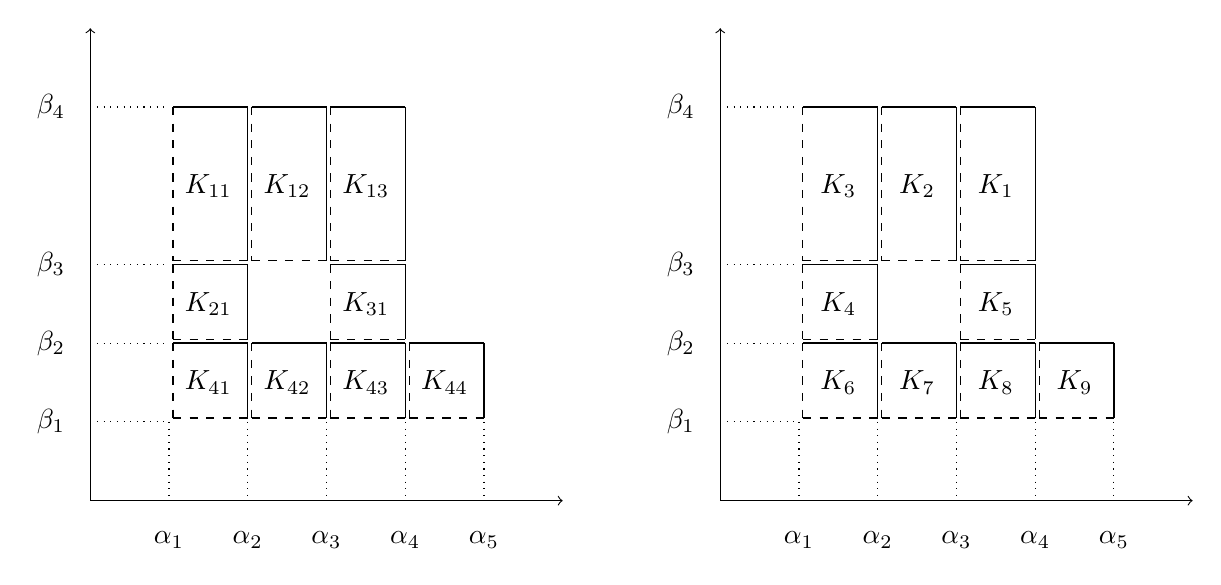
\begin{tikzpicture}[auto]
    \draw[line width=0.5pt] (10.05,3)--(11,3);
    \draw[line width=0.5pt] (11,3)--(11,2.05);
    \draw[line width=0.5pt] (11.05,3)--(12,3);
    \draw[line width=0.5pt] (12,3)--(12,2.05);
    \draw[line width=0.5pt] (12.05,3)--(13,3);
    \draw[line width=0.5pt] (13,3)--(13,2.05);
    \draw[line width=0.5pt] (13.05,3)--(14,3);
    \draw[line width=0.5pt] (14,3)--(14,2.05);
    \draw[line width=0.5pt] (10.05,4)--(11,4);
    \draw[line width=0.5pt] (11,4)--(11,3.05);
   
   
    \draw[line width=0.5pt] (12.05,4)--(13,4);
    \draw[line width=0.5pt] (13,4)--(13,3.05);
   
   
    \draw[line width=0.5pt] (10.05,6)--(11,6);
    \draw[line width=0.5pt] (11,6)--(11,4.05);
    \draw[line width=0.5pt] (11.05,6)--(12,6);
    \draw[line width=0.5pt] (12,6)--(12,4.05);
    \draw[line width=0.5pt] (12.05,6)--(13,6);
    \draw[line width=0.5pt] (13,6)--(13,4.05);
   
   
    \draw[dashed] (10.05,3)--(10.05,2.05);
    \draw[dashed] (10.05,2.05)--(11,2.05);
    \draw[dashed] (11.05,3)--(11.05,2.05);
    \draw[dashed] (11.05,2.05)--(12,2.05);
    \draw[dashed] (12.05,3)--(12.05,2.05);
    \draw[dashed] (12.05,2.05)--(13,2.05);
    \draw[dashed] (13.05,3)--(13.05,2.05);
    \draw[dashed] (13.05,2.05)--(14,2.05);
    \draw[dashed] (10.05,4)--(10.05,3.05);
    \draw[dashed] (10.05,3.05)--(11,3.05);
   
   
    \draw[dashed] (12.05,4)--(12.05,3.05);
    \draw[dashed] (12.05,3.05)--(13,3.05);
   
   
    \draw[dashed] (10.05,6)--(10.05,4.05);
    \draw[dashed] (10.05,4.05)--(11,4.05);
    \draw[dashed] (11.05,6)--(11.05,4.05);
    \draw[dashed] (11.05,4.05)--(12,4.05);
    \draw[dashed] (12.05,6)--(12.05,4.05);
    \draw[dashed] (12.05,4.05)--(13,4.05);
   
   
    \draw[dotted] (2,2)--(2,1);
    \draw[dotted] (3,2)--(3,1);
    \draw[dotted] (4,2)--(4,1);
    \draw[dotted] (5,2)--(5,1);
    \draw[dotted] (6,2)--(6,1);
    \draw[dotted] (1,2)--(2,2);
    \draw[dotted] (1,3)--(2,3);
    \draw[dotted] (1,4)--(2,4);
    \draw[dotted] (1,6)--(2,6);
    \draw[->] (9,1)--(15,1);
    \draw[->] (9,1)--(9,7);
    \node (aaa) at (2.5,2.5) {$K_{41} $};
    \node (aab) at (3.5,2.5) {$K_{42} $};
    \node (aac) at (4.5,2.5) {$K_{43} $};
    \node (aad) at (5.5,2.5) {$K_{44} $};
    \node (aba) at (2.5,3.5) {$K_{21} $};
   
    \node (abc) at (4.5,3.5) {$K_{31} $};
   
    \node (aca) at (2.5,5) {$K_{11} $};
    \node (acb) at (3.5,5) {$K_{12} $};
    \node (acc) at (4.5,5) {$K_{13} $};
   
    \node (ba) at (2,0.5) {$\alpha_1 $};
    \node (bb) at (3,0.5) {$\alpha_2 $};
    \node (bc) at (4,0.5) {$\alpha_3 $};
    \node (bd) at (5,0.5) {$\alpha_4 $};
    \node (be) at (6,0.5) {$\alpha_5 $};
    \node (ca) at (0.5,2) {$\beta_1 $};
    \node (cb) at (0.5,3) {$\beta_2 $};
    \node (cc) at (0.5,4) {$\beta_3 $};
    \node (cd) at (0.5,6) {$\beta_4 $};
   
   
   
    \draw[line width=0.5pt] (2.05,3)--(3,3);
    \draw[line width=0.5pt] (3,3)--(3,2.05);
    \draw[line width=0.5pt] (3.05,3)--(4,3);
    \draw[line width=0.5pt] (4,3)--(4,2.05);
    \draw[line width=0.5pt] (4.05,3)--(5,3);
    \draw[line width=0.5pt] (5,3)--(5,2.05);
    \draw[line width=0.5pt] (5.05,3)--(6,3);
    \draw[line width=0.5pt] (6,3)--(6,2.05);
    \draw[line width=0.5pt] (2.05,4)--(3,4);
    \draw[line width=0.5pt] (3,4)--(3,3.05);
   
   
    \draw[line width=0.5pt] (4.05,4)--(5,4);
    \draw[line width=0.5pt] (5,4)--(5,3.05);
   
   
    \draw[line width=0.5pt] (2.05,6)--(3,6);
    \draw[line width=0.5pt] (3,6)--(3,4.05);
    \draw[line width=0.5pt] (3.05,6)--(4,6);
    \draw[line width=0.5pt] (4,6)--(4,4.05);
    \draw[line width=0.5pt] (4.05,6)--(5,6);
    \draw[line width=0.5pt] (5,6)--(5,4.05);
   
   
    \draw[dashed] (2.05,3)--(2.05,2.05);
    \draw[dashed] (2.05,2.05)--(3,2.05);
    \draw[dashed] (3.05,3)--(3.05,2.05);
    \draw[dashed] (3.05,2.05)--(4,2.05);
    \draw[dashed] (4.05,3)--(4.05,2.05);
    \draw[dashed] (4.05,2.05)--(5,2.05);
    \draw[dashed] (5.05,3)--(5.05,2.05);
    \draw[dashed] (5.05,2.05)--(6,2.05);
    \draw[dashed] (2.05,4)--(2.05,3.05);
    \draw[dashed] (2.05,3.05)--(3,3.05);
   
   
    \draw[dashed] (4.05,4)--(4.05,3.05);
    \draw[dashed] (4.05,3.05)--(5,3.05);
   
   
    \draw[dashed] (2.05,6)--(2.05,4.05);
    \draw[dashed] (2.05,4.05)--(3,4.05);
    \draw[dashed] (3.05,6)--(3.05,4.05);
    \draw[dashed] (3.05,4.05)--(4,4.05);
    \draw[dashed] (4.05,6)--(4.05,4.05);
    \draw[dashed] (4.05,4.05)--(5,4.05);
   
   
    \draw[dotted] (10,2)--(10,1);
    \draw[dotted] (11,2)--(11,1);
    \draw[dotted] (12,2)--(12,1);
    \draw[dotted] (13,2)--(13,1);
    \draw[dotted] (14,2)--(14,1);
    \draw[dotted] (9,2)--(10,2);
    \draw[dotted] (9,3)--(10,3);
    \draw[dotted] (9,4)--(10,4);
    \draw[dotted] (9,6)--(10,6);
    \draw[->] (1,1)--(7,1);
    \draw[->] (1,1)--(1,7);
    \node (aaa) at (10.5,2.5) {$K_{6} $};
    \node (aab) at (11.5,2.5) {$K_{7} $};
    \node (aac) at (12.5,2.5) {$K_{8} $};
    \node (aad) at (13.5,2.5) {$K_{9} $};
    \node (aba) at (10.5,3.5) {$K_{4} $};
   
    \node (abc) at (12.5,3.5) {$K_{5} $};
   
    \node (aca) at (10.5,5) {$K_{3} $};
    \node (acb) at (11.5,5) {$K_{2} $};
    \node (acc) at (12.5,5) {$K_{1} $};
   
    \node (ba) at (10,0.5) {$\alpha_1 $};
    \node (bb) at (11,0.5) {$\alpha_2 $};
    \node (bc) at (12,0.5) {$\alpha_3 $};
    \node (bd) at (13,0.5) {$\alpha_4 $};
    \node (be) at (14,0.5) {$\alpha_5 $};
    \node (ca) at (8.5,2) {$\beta_1 $};
    \node (cb) at (8.5,3) {$\beta_2 $};
    \node (cc) at (8.5,4) {$\beta_3 $};
    \node (cd) at (8.5,6) {$\beta_4 $};
   
   
   
  \end{tikzpicture}
\end{center}
次式が得られる。
\begin{align*}
\sum_{i \in \varLambda_{m}} {\psi_{F}\left( I_{i} \right)} = \sum_{i \in \varLambda_{p}} {\psi_{F}\left( K_{i} \right)}
\end{align*}
同様にして、次式が得られる。
\begin{align*}
\sum_{j \in \varLambda_{n}} {\psi_{F}\left( J_{j} \right)} = \sum_{i \in \varLambda_{p}} {\psi_{F}\left( K_{i} \right)}
\end{align*}
よって、次式が成り立つ。
\begin{align*}
\varPsi_{F}(E) = \sum_{i \in \varLambda_{m}} {\psi_{F}\left( I_{i} \right)} = \sum_{j \in \varLambda_{n}} {\psi_{F}\left( J_{j} \right)}
\end{align*}
\end{proof}
\begin{thm}\label{4.5.4.4}
上で定義された写像$\varPsi_{F}:\mathfrak{F}_{n} \rightarrow \mathrm{cl}\mathbb{R}^{+}$はJordan測度である。
\end{thm}
\begin{proof}
上で定義された写像$\varPsi_{F}:\mathfrak{F}_{n} \rightarrow \mathrm{cl}\mathbb{R}^{+}$について、その集合$\mathfrak{F}_{n}$は定義より明らかに有限加法族となっており$V\left( \varPsi_{F} \right) \subseteq \mathrm{cl}\mathbb{R}^{+}$が成り立つ。また、定理\ref{4.5.4.1}中の定義より$\varPsi_{F}(\emptyset) = 0$が成り立つ。さらに、定理\ref{4.5.4.2}中の定義より明らかに有限加法的である。したがって、その写像$\varPsi_{F}:\mathfrak{F}_{n} \rightarrow \mathrm{cl}\mathbb{R}^{+}$はJordan測度である。
\end{proof}
%\hypertarget{lebesgue-stieltjesux6e2cux5ea6}{%
\subsubsection{Lebesgue-Stieltjes測度}%\label{lebesgue-stieltjesux6e2cux5ea6}}
\begin{thm}\label{4.5.4.5}
関数$F:\mathbb{R} \rightarrow \mathbb{R}^{n}$についての有限加法的なLebesgue-Stieltjes測度$\varPsi_{F}:\mathfrak{F}_{n} \rightarrow \mathrm{cl}\mathbb{R}^{+}$がその集合$\mathfrak{F}_{n}$上で完全加法的であるならそのときに限り、$F = \left( f_{i} \right)_{i \in \varLambda_{n}}$、$\mathbf{x} = \left( x_{i} \right)_{i \in \varLambda_{n}}$として、$\forall i \in \varLambda_{n}\forall\mathbf{x} \in \mathfrak{F}_{n}$に対し、それらの関数たち$f_{i}$がその元$x_{i}$で右連続である。
\end{thm}\par
これは次のようにして示される。
\begin{enumerate}
\item
  その有限加法的なLebesgue-Stieltjes測度$\varPsi_{F}:\mathfrak{F}_{n} \rightarrow \mathrm{cl}\mathbb{R}^{+}$がその集合$\mathfrak{F}_{n}$上で完全加法的であるとする。
\item
  $\forall i \in \varLambda_{n}\forall a \in \mathbb{R}$に対し、次のことを満たすような任意の実数列$\left( \lambda_{m} \right)_{m \in \mathbb{N}}$と
  \begin{itemize}
  \item
    $\forall m \in \mathbb{N}$に対し、$\lambda_{m + 1} < \lambda_{m}$が成り立つ。
  \item
    $\forall m \in \mathbb{N}$に対し、$a < \lambda_{m}$が成り立つ。
  \item
    $m \rightarrow \infty$のとき、$\lambda_{m} \rightarrow a$が成り立つ。
  \end{itemize}
  次式のように集合$I_{m}$、$I$が考えられる。
  \begin{align*}
  I_{m} &= \prod_{k \in \varLambda_{i - 1}} \left( a_{k},b_{k} \right] \times \left( \lambda_{m + 1},\lambda_{m} \right] \times \prod_{k \in \varLambda_{n} \setminus \varLambda_{i}} \left( a_{k},b_{k} \right]\\
  I &= \prod_{k \in \varLambda_{i - 1}} \left( a_{k},b_{k} \right] \times \left( a,\lambda_{1} \right] \times \prod_{k \in \varLambda_{n} \setminus \varLambda_{i}} \left( a_{k},b_{k} \right]
  \end{align*}
\item
  次式が成り立つことが示される。
  \begin{align*}
  \varPsi_{F}(I) = \lim_{m \rightarrow \infty}{\sum_{l \in \varLambda_{m - 1}} {\varPsi_{F}\left( I_{l} \right)}}
  \end{align*}
\item
  これにより、次式が成り立つことが示される。
  \begin{align*}
  f_{i}\left( \lambda_{1} \right) - f_{i}(a) = f_{i}\left( \lambda_{1} \right) - \lim_{\lambda_{m} \rightarrow a + 0}{f_{i}\left( \lambda_{m} \right)}
  \end{align*}
\item
  1. から4. よりよって、それらの関数たち$f_{i}$は右連続であることが示された。
\item
  逆に、上のように仮定されるとする。
\item
  まず、$\forall I \in \mathfrak{I}_{n}\forall\alpha < \varPsi_{F}(I)\exists J \in \mathfrak{I}_{n}$に対し、その区間$J$が有界で次式が成り立つことを示そう。
  \begin{align*}
  \mathrm{cl}J \subseteq I,\ \ \alpha < \varPsi_{F}(J)
  \end{align*}
\item
  $0 \leq \alpha$で考え$I = \prod_{i \in \varLambda_{n}} \left( a_{i},b_{i} \right]$と与えられたとし、$\forall i \in \varLambda_{n}$に対し、次のことを満たすような実数列たち$\left( a_{m,i} \right)_{i \in \varLambda_{n}}$、$\left( b_{m,i} \right)_{i \in \varLambda_{n}}$が考えれられよう。
  \begin{itemize}
  \item
    $\forall i \in \varLambda_{n}$に対し、その実数列$\left( a_{m,i} \right)_{m \in \mathbb{N}}$は狭義単調減少し次式が成り立つ。
  \begin{align*}
  \lim_{m \rightarrow \infty}a_{m,i} = a_{i}
  \end{align*}
  \item
    $\forall i \in \varLambda_{n}$に対し、$b_{i} < \infty$のとき、$\left( b_{m,i} \right)_{m \in \mathbb{N}} = b_{i}:m \mapsto b_{i}$と一定で、$b_{i} = \infty$のとき、その実数列$\left( b_{m,i} \right)_{m \in \mathbb{N}}$は狭義単調増加し正の無限大に発散する。
  \item
    $a_{1,i} < b_{1,i}$が成り立つ。
  \end{itemize}
\item
  明らかに$\mathrm{cl}{\prod_{i \in \varLambda_{n}} \left( a_{m,i},b_{m,i} \right]} \subseteq \prod_{i \in \varLambda_{n}} \left( a_{i},b_{i} \right]$が成り立つ。
\item
  愚直に計算することで、$I_{m} = \prod_{i \in \varLambda_{n}} \left( a_{m,i},b_{m,i} \right]$として、$\lim_{m \rightarrow \infty}{\varPsi_{F}\left( I_{m} \right)} = \varPsi_{F}(I)$が成り立つ。
\item
  10. よりある自然数$m$が存在して、$\alpha < \varPsi_{F}\left( I_{m} \right)$が成り立つので、このような区間$I_{m}$を$J$とすればよい。
\item
  8. ~11. で7. が示された。
\item
  次に、$\forall E \in \mathfrak{F}_{n}\forall\alpha < \varPsi_{F}(E)\exists G \in \mathfrak{F}_{n}$に対し、その区間塊$G$が有界で次式が成り立つことを示そう。
  \begin{align*}
  \mathrm{cl}G \subseteq E,\ \ \alpha < \varPsi_{F}(G)
  \end{align*}
\item
  $\forall i \in \varLambda_{m}$に対し、$\varPsi_{F}\left( I_{i} \right) < \infty$が成り立つとき、有界な区間$J_{i}$が存在して、$\mathrm{cl}J_{i} \subseteq I_{i}$かつ$\varPsi_{F}\left( I_{i} \right) - \frac{1}{m}\left( \varPsi_{F}(E) - \alpha \right) < \varPsi_{F}\left( J_{i} \right)$が成り立つ。
\item
  さらに、その和集合$\bigsqcup_{i \in \varLambda_{m}} J_{i}$は有界でその集合$\mathfrak{F}_{n}$に属し次式を満たす。
  \begin{align*}
  \mathrm{cl}{\bigsqcup_{i \in \varLambda_{m}} J_{i}} \subseteq E
  \end{align*}
\item
  計算することにより$\alpha < \varPsi_{F}\left( \bigsqcup_{i \in \varLambda_{m}} J_{i} \right)$が成り立つので、このような区間塊$\bigsqcup_{i \in \varLambda_{m}} J_{i}$を$G$とすればよい。
\item
  $\exists i \in \varLambda_{m}$に対し、$\varPsi_{F}\left( I_{i} \right) = \infty$が成り立つとき、7.
  により明らかである。
\item
  14. ~17. より13. が示された。
\item
  次に、区間塊$E$が与えられたとき、その集合$\mathfrak{I}_{n}$の元の族$\left\{ I_{m} \right\}_{m \in \mathbb{N}}$がその区間塊$E$を掩うなら、次式が成り立つことを示そう。
  \begin{align*}
  \varPsi_{F}(E) \leq \sum_{m \in \mathbb{N}} {\varPsi_{F}\left( I_{m} \right)}
  \end{align*}
\item
  それらの関数たち$f_{i}$が右連続であるから、$I_{m} = \prod_{i \in \varLambda_{n}} \left( a_{m,i},b_{m,i} \right]$として$\forall\varepsilon \in \mathbb{R}^{+}\exists\delta_{m} \in \mathbb{R}^{+}$に対し、次式が成り立つ。
  \begin{align*}
  \varPsi_{F}\left( \prod_{i \in \varLambda_{n}} \left( a_{m,i},b_{m,i} + \delta_{m} \right] \right) \leq \frac{\varepsilon}{2^{m}} + \varPsi_{F}\left( I_{m} \right)
  \end{align*}
\item
  13. により$\forall\alpha < \varPsi_{F}(E)$に対し、有界な区間塊$G$が存在して、$\mathrm{cl}G \subseteq E$かつ$\alpha < \varPsi_{F}(G)$が成り立つ。Heine-Borelの被覆定理よりその集合$\mathrm{cl}G$はcompactであるから、次式が成り立つ。
  \begin{align*}
  G \subseteq \mathrm{cl}G \subseteq \bigcup_{m \in \varLambda_{N}} {\prod_{i \in \varLambda_{n}} \left( a_{m,i},b_{m,i} + \delta_{m} \right]}
  \end{align*}
\item
  愚直に計算することで、$\alpha < \sum_{m \in \mathbb{N}} {\varPsi_{F}\left( I_{m} \right)} + \varepsilon$が成り立つ。
\item
  $\alpha + \varepsilon' - \varepsilon = \varPsi_{F}(E)$とおけば、$\varPsi_{F}(E) < \sum_{m \in \mathbb{N}} {\varPsi_{F}\left( I_{m} \right)} + \varepsilon'$が成り立つ。
\item
  20. ~23. より19. が示された。
\item
  その集合$\mathfrak{F}_{n}$の元の列$\left( E_{m} \right)_{m \in \mathbb{N}}$が与えられどの区間塊$E_{m}$も互いに素なら、$\forall m \in \mathbb{N}$に対し、ある区間の族$\mathfrak{E}_{m} = \left\{ I_{m,i} \right\}_{i \in \varLambda_{N_{m}}}$が存在して、$E_{m} = \bigsqcup_{} \mathfrak{E}_{m}$が成り立つので、次式が成り立つ。
  \begin{align*}
  \varPsi_{F}\left( E_{m} \right) = \sum_{i \in \varLambda_{N_{m}}} {\varPsi_{F}\left( I_{m,i} \right)}
  \end{align*}
\item
  19. より次式が成り立つ。
  \begin{align*}
  \varPsi_{F}\left( \bigsqcup_{m \in \mathbb{N}} E_{m} \right) \leq \sum_{m \in \mathbb{N}} {\varPsi_{F}\left( E_{m} \right)}
  \end{align*}
\item
  $\forall M \in \mathbb{N}$に対し、次式が成り立つ。
  \begin{align*}
  \sum_{m \in \varLambda_{M}} {\varPsi_{F}\left( E_{m} \right)} \leq \varPsi_{F}\left( \bigsqcup_{m \in \mathbb{N}} E_{m} \right)
  \end{align*}
\item
  $M \rightarrow \infty$とすれば、次式が成り立つ。
  \begin{align*}
  \varPsi_{F}\left( \bigsqcup_{m \in \mathbb{N}} E_{m} \right) = \sum_{m \in \mathbb{N}} {\varPsi_{F}\left( E_{m} \right)}
  \end{align*}
\item
  6. ように仮定されたとき、7. ~28. よりその有限加法的なLebesgue-Stieltjes測度$\varPsi_{F}$は完全加法的であることが示された。
\end{enumerate}
\begin{proof}
関数$F = \left( f_{i} \right)_{i \in \varLambda_{n}}:\mathbb{R} \rightarrow \mathbb{R}^{n}$についての有限加法的なLebesgue-Stieltjes測度$\varPsi_{F}:\mathfrak{F}_{n} \rightarrow \mathrm{cl}\mathbb{R}^{+}$がその集合$\mathfrak{F}_{n}$上で完全加法的であるとする。$\forall i \in \varLambda_{n}\forall a \in \mathbb{R}$に対し、次のことを満たすような任意の実数列$\left( \lambda_{m} \right)_{m \in \mathbb{N}}$が考えれられれば、
\begin{itemize}
\item
  $\forall m \in \mathbb{N}$に対し、$\lambda_{m + 1} < \lambda_{m}$が成り立つ。
\item
  $\forall m \in \mathbb{N}$に対し、$a < \lambda_{m}$が成り立つ。
\item
  $m \rightarrow \infty$のとき、$\lambda_{m} \rightarrow a$が成り立つ。
\end{itemize}
$\forall k \in \varLambda_{n}$に対し、それらの関数たち$f_{k}$は狭義単調増加するので、$- \infty < f_{k}\left( a_{k} \right) < f_{k}\left( b_{k} \right) < \infty$かつ$a_{k} < b_{k}$なる実数たち$a_{k}$、$b_{k}$が存在する。ここで、次式のように集合$I_{m}$、$I$が考えられれば、
\begin{align*}
I_{m} &= \prod_{k \in \varLambda_{i - 1}} \left( a_{k},b_{k} \right] \times \left( \lambda_{m + 1},\lambda_{m} \right] \times \prod_{k \in \varLambda_{n} \setminus \varLambda_{i}} \left( a_{k},b_{k} \right]\\
I &= \prod_{k \in \varLambda_{i - 1}} \left( a_{k},b_{k} \right] \times \left( a,\lambda_{1} \right] \times \prod_{k \in \varLambda_{n} \setminus \varLambda_{i}} \left( a_{k},b_{k} \right]
\end{align*}
$I_{m},I \in \mathfrak{I}_{n} \subseteq \mathfrak{F}_{n}$が成り立つかつ、$\left( a,\lambda_{1} \right] = \bigsqcup_{m \in \mathbb{N}} \left( \lambda_{m + 1},\lambda_{m} \right]$より$I = \bigsqcup_{m \in \mathbb{N}} I_{m}$が成り立つので、その有限加法的なLebesgue-Stieltjes測度$\varPsi_{F}$が完全加法的なことにより次のようになる。
\begin{align*}
\varPsi_{F}(I) = \varPsi_{F}\left( \bigsqcup_{m \in \mathbb{N}} I_{m} \right) = \sum_{m \in \mathbb{N}} {\varPsi_{F}\left( I_{m} \right)} = \lim_{m \rightarrow \infty}{\sum_{l \in \varLambda_{m - 1}} {\varPsi_{F}\left( I_{l} \right)}}
\end{align*}
ここで、次のように実数$M$が考えられれば、
\begin{align*}
M = \prod_{k \in \varLambda_{n} \setminus \left\{ i \right\}} \left( f_{k}\left( b_{k} \right) - f_{k}\left( a_{k} \right) \right)
\end{align*}
$0 < M$が成り立つので、次のようになる。
\begin{align*}
\varPsi_{F}\left( I_{l} \right) &= \prod_{k \in \varLambda_{i - 1}} \left( f_{k}\left( b_{k} \right) - f_{k}\left( a_{k} \right) \right)\left( f_{i}\left( \lambda_{l} \right) - f_{i}\left( \lambda_{l + 1} \right) \right)\prod_{k \in \varLambda_{n} \setminus \varLambda_{i}} \left( f_{k}\left( b_{k} \right) - f_{k}\left( a_{k} \right) \right)\\
&= \left( f_{i}\left( \lambda_{l} \right) - f_{i}\left( \lambda_{l + 1} \right) \right)\prod_{k \in \varLambda_{n} \setminus \left\{ i \right\}} \left( f_{k}\left( b_{k} \right) - f_{k}\left( a_{k} \right) \right)\\
&= \left( f_{i}\left( \lambda_{l} \right) - f_{i}\left( \lambda_{l + 1} \right) \right)M\\
\varPsi_{F}(I) &= \prod_{k \in \varLambda_{i - 1}} \left( f_{k}\left( b_{k} \right) - f_{k}\left( a_{k} \right) \right)\left( f_{i}\left( \lambda_{1} \right) - f_{i}(a) \right)\prod_{k \in \varLambda_{n} \setminus \varLambda_{i}} \left( f_{k}\left( b_{k} \right) - f_{k}\left( a_{k} \right) \right)\\
&= \left( f_{i}\left( \lambda_{1} \right) - f_{i}(a) \right)\prod_{k \in \varLambda_{n} \setminus \left\{ i \right\}} \left( f_{k}\left( b_{k} \right) - f_{k}\left( a_{k} \right) \right)\\
&= \left( f_{i}\left( \lambda_{1} \right) - f_{i}(a) \right)M
\end{align*}
したがって、次のようになる。
\begin{align*}
f_{i}\left( \lambda_{1} \right) - f_{i}(a) &= \frac{1}{M}\left( f_{i}\left( \lambda_{1} \right) - f_{i}(a) \right)M\\
&= \frac{1}{M}\varPsi_{F}(I)\\
&= \frac{1}{M}\lim_{m \rightarrow \infty}{\sum_{l \in \varLambda_{m - 1}} {\varPsi_{F}\left( I_{l} \right)}}\\
&= \frac{1}{M}\lim_{m \rightarrow \infty}{\sum_{l \in \varLambda_{m - 1}} {\left( f_{i}\left( \lambda_{l} \right) - f_{i}\left( \lambda_{l + 1} \right) \right)M}}\\
&= \lim_{m \rightarrow \infty}{\sum_{l \in \varLambda_{m - 1}} \left( f_{i}\left( \lambda_{l} \right) - f_{i}\left( \lambda_{l + 1} \right) \right)}\\
&= \lim_{m \rightarrow \infty}\left( f_{i}\left( \lambda_{1} \right) - f_{i}\left( \lambda_{m} \right) \right)\\
&= f_{i}\left( \lambda_{1} \right) - \lim_{m \rightarrow \infty}{f_{i}\left( \lambda_{m} \right)}\\
&= f_{i}\left( \lambda_{1} \right) - \lim_{\lambda_{m} \rightarrow a + 0}{f_{i}\left( \lambda_{m} \right)}
\end{align*}
よって、$\lim_{\lambda_{m} \rightarrow a + 0}{f_{i}\left( \lambda_{m} \right)} = f_{i}(a)$が成り立つので、$\mathbf{x} = \left( x_{i} \right)_{i \in \varLambda_{n}}$として、$\forall i \in \varLambda_{n}\forall\mathbf{x} \in \mathfrak{F}_{n}$に対し、それらの関数たち$f_{i}$はその元$x_{i}$で右連続である。\par
逆に、$\mathbf{x} = \left( x_{i} \right)_{i \in \varLambda_{n}}$として、$\forall i \in \varLambda_{n}\forall\mathbf{x} \in \mathfrak{F}_{n}$に対し、それらの関数たち$f_{i}$はその元$x_{i}$で右連続であるとする。\par
ここでまず、$\forall I \in \mathfrak{I}_{n}\forall\alpha < \varPsi_{F}(I)\exists J \in \mathfrak{I}_{n}$に対し、その区間$J$が有界で次式が成り立つことを示そう。
\begin{align*}
\mathrm{cl}J \subseteq I,\ \ \alpha < \varPsi_{F}(J)
\end{align*}
$\alpha < 0$のときでは$J = \emptyset$とすればよいので、$0 \leq \alpha$で考えよう。$I = \prod_{i \in \varLambda_{n}} \left( a_{i},b_{i} \right]$と与えられたとし、さらに、$\mathbf{a}_{m} = \left( a_{m,i} \right)_{i \in \varLambda_{n}}$、$\mathbf{b}_{m} = \left( b_{m,i} \right)_{i \in \varLambda_{n}}$、$I_{m} = \prod_{i \in \varLambda_{n}} \left( a_{m,i},b_{m,i} \right]$として、次のことを満たすような点列たち$\left( \mathbf{a}_{m} \right)_{m \in \mathbb{N}}$、$\left( \mathbf{b}_{m} \right)_{m \in \mathbb{N}}$が考えれられれば、
\begin{itemize}
\item
  $\forall i \in \varLambda_{n}$に対し、その実数列$\left( a_{m,i} \right)_{m \in \mathbb{N}}$は狭義単調減少し次式が成り立つ。
  \begin{align*}
  \lim_{m \rightarrow \infty}a_{m,i} = a_{i}
  \end{align*}
\item
  $\forall i \in \varLambda_{n}$に対し、$b_{i} < \infty$のとき、$\left( b_{m,i} \right)_{m \in \mathbb{N}} = b_{i}:m \mapsto b_{i}$と一定で、$b_{i} = \infty$のとき、その実数列$\left( b_{m,i} \right)_{m \in \mathbb{N}}$は狭義単調増加し正の無限大に発散する。
\item
  $a_{1,i} < b_{1,i}$が成り立つ。
\end{itemize}
$\forall i \in \varLambda_{n}$に対し、$a_{i} < a_{m,i} < a_{1,i} < b_{1,i} < b_{m,i} < b_{i}$が成り立つことから、次式が成り立ち、
\begin{align*}
\mathrm{cl}{\prod_{i \in \varLambda_{n}} \left( a_{m,i},b_{m,i} \right]} = \prod_{i \in \varLambda_{n}} \left[ a_{m,i},b_{m,i} \right] \subseteq \prod_{i \in \varLambda_{n}} \left( a_{i},b_{i} \right]
\end{align*}
$\alpha < \varPsi_{F}(I)$が成り立つことから、$\forall i \in \varLambda_{n}$に対し、その差$f_{i}\left( b_{i} \right) - f_{i}\left( a_{i} \right)$が$0$でありえなく、$m \rightarrow \infty$のとき、その差$f_{i}\left( b_{m,i} \right) - f_{i}\left( a_{m,i} \right)$も$0$でない正の実数か$\infty$に広い意味で収束するので、したがって、次のようになる。
\begin{align*}
\lim_{m \rightarrow \infty}{\varPsi_{F}\left( I_{m} \right)} &= \lim_{m \rightarrow \infty}{\varPsi_{F}\left( \prod_{i \in \varLambda_{n}} \left( a_{m,i},b_{m,i} \right] \right)}\\
&= \lim_{m \rightarrow \infty}{\prod_{i \in \varLambda_{n}} \left( f_{i}\left( b_{m,i} \right) - f_{i}\left( a_{m,i} \right) \right)}\\
&= \prod_{i \in \varLambda_{n}} {\lim_{m \rightarrow \infty}\left( f_{i}\left( b_{m,i} \right) - f_{i}\left( a_{m,i} \right) \right)}\\
&= \left\{ \begin{matrix}
\prod_{i \in \varLambda_{n}} {\lim_{\scriptsize \begin{matrix}
a_{im} \rightarrow a_{i} + 0 \\
b_{im} = b_{i} \\
\end{matrix}}\left( f_{i}\left( b_{m,i} \right) - f_{i}\left( a_{m,i} \right) \right)} & \mathrm{if} & b_{i} < \infty \\
\prod_{i \in \varLambda_{n}} {\lim_{\scriptsize \begin{matrix}
a_{im} \rightarrow a_{i} + 0 \\
b_{im} \rightarrow \infty \\
\end{matrix}}\left( f_{i}\left( b_{m,i} \right) - f_{i}\left( a_{m,i} \right) \right)} & \mathrm{if} & b_{i} = \infty \\
\end{matrix} \right.\ \\
&= \left\{ \begin{matrix}
\prod_{i \in \varLambda_{n}} \left( f_{i}\left( b_{i} \right) - f_{i}\left( a_{i} \right) \right) & \mathrm{if} & b_{i} < \infty \\
\prod_{i \in \varLambda_{n}} {\lim_{\scriptsize \begin{matrix}
b_{im} \rightarrow \infty \\
\end{matrix}}\left( f_{i}\left( b_{m,i} \right) - f_{i}\left( a_{i} \right) \right)} & \mathrm{if} & b_{i} = \infty \\
\end{matrix} \right.\ \\
&= \left\{ \begin{matrix}
\prod_{i \in \varLambda_{n}} \left( f_{i}\left( b_{i} \right) - f_{i}\left( a_{i} \right) \right) & \mathrm{if} & b_{i} < \infty \\
\prod_{i \in \varLambda_{n}} \left( f_{i}\left( b_{i} \right) - f_{i}\left( a_{i} \right) \right) & \mathrm{if} & b_{i} = \infty \\
\end{matrix} \right.\ \\
&= \prod_{i \in \varLambda_{n}} \left( f_{i}\left( b_{i} \right) - f_{i}\left( a_{i} \right) \right)\\
&= \varPsi_{F}(I)
\end{align*}
したがって、$\forall\varepsilon \in \mathbb{R}^{+}$に対し、$\varPsi_{F}(I) < \infty$のとき、$\varepsilon < \varPsi_{F}(I) - \alpha$とすれば、$\exists N \in \mathbb{N}\forall m \in \mathbb{N}$に対し、$N \leq m$が成り立つなら、次のようになる。
\begin{align*}
\left| \varPsi_{F}\left( I_{m} \right) - \varPsi_{F}(I) \right| < \varepsilon &\Leftrightarrow - \varepsilon < \varPsi_{F}\left( I_{m} \right) - \varPsi_{F}(I) < \varepsilon\\
&\Leftrightarrow \alpha < \varPsi_{F}(I) - \varepsilon < \varPsi_{F}\left( I_{m} \right) < \varPsi_{F}(I) + \varepsilon\\
&\Rightarrow \alpha < \varPsi_{F}\left( I_{m} \right)
\end{align*}
このような自然数$m$で考えられれば、$\alpha < \varPsi_{F}\left( I_{m} \right)$が成り立つので、このような区間$I_{m}$を$J$とすればよい。$\varPsi_{F}(I) = \infty$のとき、$\varepsilon = \alpha$とすれば、$\exists N \in \mathbb{N}\forall m \in \mathbb{N}$に対し、$N \leq m$が成り立つなら、次のようになる。
\begin{align*}
\alpha = \varepsilon < \varPsi_{F}\left( \prod_{i \in \varLambda_{n}} \left( a_{m,i},b_{m,i} \right] \right)
\end{align*}
このような自然数$m$で考えられれば、$\alpha < \varPsi_{F}\left( \prod_{i \in \varLambda_{n}} \left( a_{m,i},b_{m,i} \right] \right)$が成り立つので、このような区間$\prod_{i \in \varLambda_{n}} \left( a_{m,i},b_{m,i} \right]$を$J$とすればよい。\par
次に、$\forall E \in \mathfrak{F}_{n}\forall\alpha < \varPsi_{F}(E)\exists G \in \mathfrak{F}_{n}$に対し、その区間塊$G$が有界で次式が成り立つことを示そう。
\begin{align*}
\mathrm{cl}G \subseteq E,\ \ \alpha < \varPsi_{F}(G)
\end{align*}
区間塊の定義よりその集合$\mathfrak{I}_{n}$の元の族$\left\{ I_{i} \right\}_{i \in \varLambda_{m}}$を用いて$E = \bigsqcup_{i \in \varLambda_{m}} I_{i}$と与えられることができる。$\forall i \in \varLambda_{m}$に対し、$\varPsi_{F}\left( I_{i} \right) < \infty$が成り立つとき、上記の議論により有界な区間$J_{i}$が存在して、$\mathrm{cl}J_{i} \subseteq I_{i}$かつ$\varPsi_{F}\left( I_{i} \right) - \frac{1}{m}\left( \varPsi_{F}(E) - \alpha \right) < \varPsi_{F}\left( J_{i} \right)$が成り立つ。このとき、それらの区間たち$J_{i}$は互いに素でその和集合$\bigsqcup_{i \in \varLambda_{m}} J_{i}$は有界でその集合$\mathfrak{F}_{n}$に属し次式を満たす。
\begin{align*}
\mathrm{cl}{\bigsqcup_{i \in \varLambda_{m}} J_{i}} = \bigsqcup_{i \in \varLambda_{m}} {\mathrm{cl}J_{i}} \subseteq \bigsqcup_{i \in \varLambda_{m}} I_{i} = E
\end{align*}
さらに、次のようになる。
\begin{align*}
\varPsi_{F}\left( \bigsqcup_{i \in \varLambda_{m}} J_{i} \right) &= \sum_{i \in \varLambda_{m}} {\varPsi_{F}\left( J_{i} \right)}\\
&> \sum_{i \in \varLambda_{m}} \left( \varPsi_{F}\left( I_{i} \right) - \frac{1}{m}\left( \varPsi_{F}(E) - \alpha \right) \right)\\
&= \sum_{i \in \varLambda_{m}} {\varPsi_{F}\left( I_{i} \right)} - \sum_{i \in \varLambda_{m}} {\frac{1}{m}\left( \varPsi_{F}(E) - \alpha \right)}\\
&= \sum_{i \in \varLambda_{m}} {\varPsi_{F}\left( I_{i} \right)} - \frac{m}{m}\left( \varPsi_{F}(E) - \alpha \right)\\
&= \sum_{i \in \varLambda_{m}} {\varPsi_{F}\left( I_{i} \right)} - \varPsi_{F}(E) + \alpha\\
&= \varPsi_{F}\left( \bigsqcup_{i \in \varLambda_{m}} I_{i} \right) - \varPsi_{F}\left( \bigsqcup_{i \in \varLambda_{m}} I_{i} \right) + \alpha\\
&= \alpha
\end{align*}
これにより、$\alpha < \varPsi_{F}\left( \bigsqcup_{i \in \varLambda_{m}} J_{i} \right)$が成り立つので、このような区間塊$\bigsqcup_{i \in \varLambda_{m}} J_{i}$を$G$とすればよい。$\exists i \in \varLambda_{m}$に対し、$\varPsi_{F}\left( I_{i} \right) = \infty$が成り立つとき、上記の議論により有界な区間$J_{i}$が存在して、$\mathrm{cl}J_{i} \subseteq I_{i}$かつ$\alpha < \varPsi_{F}\left( J_{i} \right)$が成り立つ。このとき、$\mathrm{cl}J_{i} \subseteq I_{i} \subseteq E$かつ$\alpha < \varPsi_{F}\left( J_{i} \right)$が成り立つ。このような区間$J_{i}$を$G$とすればよい。\par
次に、区間塊$E$が与えられたとき、その集合$\mathfrak{I}_{n}$の元の族$\left\{ I_{m} \right\}_{m \in \mathbb{N}}$がその区間塊$E$を掩うなら、次式が成り立つことを示そう。
\begin{align*}
\varPsi_{F}(E) \leq \sum_{m \in \mathbb{N}} {\varPsi_{F}\left( I_{m} \right)}
\end{align*}
このとき、$\forall m \in \mathbb{N}$に対し、$J_{m} = \prod_{i \in \varLambda_{n}} \left( a_{m,i}',b_{m,i}' \right] \subseteq I_{m}$かつ$a_{m,i}',b_{m,i}' \in \mathbb{R}$なる任意の区間$J_{m}$に対し、それらの関数たち$f_{i}$が右連続であるから、$\forall\varepsilon \in \mathbb{R}^{+}\exists\delta_{m} \in \mathbb{R}^{+}$に対し、$0 \leq x_{i} - b_{m,i}' < 2\delta_{m}$が成り立つなら、次式が成り立つ。
\begin{align*}
f_{i}\left( x_{i} \right) - f_{i}\left( b_{m,i}' \right) < \frac{\varepsilon}{n2^{m}M},\ \ M = \prod_{i \in \varLambda_{n}} \left( f_{i}\left( b_{m,i}' + \delta_{m} \right) - f_{i}\left( a_{m,i}' \right) \right)
\end{align*}
特に、次式が成り立つ。
\begin{align*}
f_{i}\left( b_{m,i}' + \delta_{m} \right) - f_{i}\left( b_{m,i}' \right) < \frac{\varepsilon}{n2^{m}M}
\end{align*}
したがって、次のようになる。
\begin{align*}
&\quad \prod_{i \in \varLambda_{n}} \left( f_{i}\left( b_{m,i}' + \delta_{m} \right) - f_{i}\left( a_{m,i}' \right) \right) - \prod_{i \in \varLambda_{n}} \left( f_{i}\left( b_{m,i}' \right) - f_{i}\left( a_{m,i}' \right) \right)\\
&\leq \sum_{i \in \varLambda_{n}} {\left( f_{i}\left( b_{m,i}' + \delta_{m} \right) - f_{i}\left( b_{m,i}' \right) \right)\prod_{j \in \varLambda_{n} \setminus \left\{ i \right\}} \left( f_{j}\left( b_{m,j}' + \delta_{m} \right) - f_{j}\left( a_{m,j}' \right) \right)}\\
&\leq \sum_{i \in \varLambda_{n}} {\left( f_{i}\left( b_{m,i}' + \delta_{m} \right) - f_{i}\left( b_{m,i}' \right) \right)\prod_{j \in \varLambda_{n}} \left( f_{j}\left( b_{m,j}' + \delta_{m} \right) - f_{j}\left( a_{m,j}' \right) \right)}\\
&= M\sum_{i \in \varLambda_{n}} \left( f_{i}\left( b_{m,i}' + \delta_{m} \right) - f_{i}\left( b_{m,i}' \right) \right)\\
&< M\sum_{j \in \varLambda_{n}} \frac{\varepsilon}{n2^{m}M} = M\frac{\varepsilon}{n2^{m}M}n = \frac{\varepsilon}{2^{m}}
\end{align*}
したがって、次式が成り立つ。
\begin{align*}
\prod_{i \in \varLambda_{n}} \left( f_{i}\left( b_{m,i}' + \delta_{m} \right) - f_{i}\left( a_{m,i}' \right) \right) \leq \frac{\varepsilon}{2^{m}} + \prod_{i \in \varLambda_{n}} \left( f_{i}\left( b_{m,i}' \right) - f_{i}\left( a_{m,i}' \right) \right)
\end{align*}
両辺に上限がとられれば、$I_{m} = \prod_{i \in \varLambda_{n}} \left( a_{m,i},b_{m,i} \right]$として次のようになる。
\begin{align*}
\varPsi_{F}\left( \prod_{i \in \varLambda_{n}} \left( a_{m,i},b_{m,i} + \delta_{m} \right] \right) \leq \frac{\varepsilon}{2^{m}} + \varPsi_{F}\left( \prod_{i \in \varLambda_{n}} \left( a_{m,i},b_{m,i} \right] \right) = \frac{\varepsilon}{2^{m}} + \varPsi_{F}\left( I_{m} \right)
\end{align*}
ここで、上記の議論により$\forall\alpha < \varPsi_{F}(E)$に対し、有界な区間塊$G$が存在して、$\mathrm{cl}G \subseteq E$かつ$\alpha < \varPsi_{F}(G)$が成り立つので、次のようにおかれると、
\begin{align*}
\prod_{i \in \varLambda_{n}} \left( a_{m,i},b_{m,i} + \delta_{m} \right) = G_{m}
\end{align*}
$I_{m} \subseteq G_{m} \subseteq \prod_{i \in \varLambda_{n}} \left( a_{m,i},b_{m,i} + \delta_{m} \right]$より次のようになる。
\begin{align*}
G \subseteq \mathrm{cl}G \subseteq E \subseteq \bigcup_{m \in \mathbb{N}} I_{m} \subseteq \bigcup_{m \in \mathbb{N}} G_{m} \subseteq \bigcup_{m \in \mathbb{N}} {\prod_{i \in \varLambda_{n}} \left( a_{m,i},b_{m,i} + \delta_{m} \right]}
\end{align*}
ここで、Heine-Borelの被覆定理よりその閉集合$\mathrm{cl}G$はcompactであるから、次式が成り立つ。
\begin{align*}
G \subseteq \mathrm{cl}G \subseteq \bigcup_{m \in \varLambda_{N}} G_{m} \subseteq \bigcup_{m \in \varLambda_{N}} {\prod_{i \in \varLambda_{n}} \left( a_{m,i},b_{m,i} + \delta_{m} \right]}
\end{align*}
したがって、次のようになる。
\begin{align*}
\alpha &< \varPsi_{F}(G)\\
&\leq \varPsi_{F}\left( \bigcup_{m \in \varLambda_{N}} {\prod_{i \in \varLambda_{n}} \left( a_{m,i},b_{m,i} + \delta_{m} \right]} \right)\\
&\leq \sum_{m \in \varLambda_{N}} {\varPsi_{F}\left( \prod_{i \in \varLambda_{n}} \left( a_{m,i},b_{m,i} + \delta_{m} \right] \right)}\\
&\leq \sum_{m \in \varLambda_{N}} \left( \frac{\varepsilon}{2^{m}} + \varPsi_{F}\left( I_{m} \right) \right)\\
&= \sum_{m \in \varLambda_{N}} {\varPsi_{F}\left( I_{m} \right)} + \sum_{m \in \varLambda_{N}} \frac{\varepsilon}{2^{m}}\\
&= \sum_{m \in \varLambda_{N}} {\varPsi_{F}\left( I_{m} \right)} + \frac{\varepsilon}{2}\frac{1 - \left( \frac{1}{2} \right)^{N}}{1 - \frac{1}{2}}\\
&= \sum_{m \in \varLambda_{N}} {\varPsi_{F}\left( I_{m} \right)} + \varepsilon\left( 1 - \left( \frac{1}{2} \right)^{N} \right)\\
&< \sum_{m \in \varLambda_{N}} {\varPsi_{F}\left( I_{m} \right)} + \varepsilon\\
&\leq \sum_{m \in \mathbb{N}} {\varPsi_{F}\left( I_{m} \right)} + \varepsilon
\end{align*}
したがって、$\alpha < \sum_{m \in \mathbb{N}} {\varPsi_{F}\left( I_{m} \right)} + \varepsilon$となりその実数$\alpha$はどれだけ$\varPsi_{F}(E)$の近くとれるので、$\alpha + \varepsilon' - \varepsilon = \varPsi_{F}(E)$とおけば、次式が成り立つ。
\begin{align*}
\varPsi_{F}(E) < \sum_{m \in \mathbb{N}} {\varPsi_{F}\left( I_{m} \right)} + \varepsilon'
\end{align*}
よって、区間塊$E$が与えられたとき、その集合$\mathfrak{I}_{n}$の元の族$\left\{ I_{m} \right\}_{m \in \mathbb{N}}$がその区間塊$E$を掩うなら、$\varPsi_{F}(E) \leq \sum_{m \in \mathbb{N}} {\varPsi_{F}\left( I_{m} \right)}$が成り立つ。\par
その集合$\mathfrak{F}_{n}$の元の列$\left( E_{m} \right)_{m \in \mathbb{N}}$が与えられどの区間塊$E_{m}$も互いに素なら、$\forall m \in \mathbb{N}$に対し、ある区間の族$\mathfrak{E}_{m} = \left\{ I_{m,i} \right\}_{i \in \varLambda_{N_{m}}}$が存在して、$E_{m} = \bigsqcup_{} \mathfrak{E}_{m}$が成り立つので、次式が成り立つ。
\begin{align*}
\varPsi_{F}\left( E_{m} \right) = \sum_{i \in \varLambda_{N_{m}}} {\varPsi_{F}\left( I_{m,i} \right)}
\end{align*}
このとき、上記の議論によりその集合$\mathfrak{I}_{n}$の元の族$\bigcup_{m \in \mathbb{N}} \mathfrak{E}_{m}$がその区間塊$\bigsqcup_{m \in \mathbb{N}} E_{m}$を掩うので、次式が成り立つ。
\begin{align*}
\varPsi_{F}\left( \bigsqcup_{m \in \mathbb{N}} E_{m} \right) \leq \sum_{\scriptsize \begin{matrix}
i \in \varLambda_{N_{m}} \\
m \in \mathbb{N} \\
\end{matrix}} {{\varPsi_{F}}_{F}\left( I_{m,i} \right)} = \sum_{m \in \mathbb{N}} {\sum_{\scriptsize \begin{matrix}
i \in \varLambda_{N_{m}} \\
\end{matrix}} {\varPsi_{F}\left( I_{m,i} \right)}} = \sum_{m \in \mathbb{N}} {\varPsi_{F}\left( E_{m} \right)}
\end{align*}
一方で、$\forall M \in \mathbb{N}$に対し、$\bigsqcup_{m \in \varLambda_{M}} E_{m} \subseteq \bigsqcup_{m \in \mathbb{N}} E_{m}$が成り立つので、次のようになり、
\begin{align*}
\varPsi_{F}\left( \bigsqcup_{m \in \varLambda_{M}} E_{m} \right) = \sum_{m \in \varLambda_{M}} {\varPsi_{F}\left( E_{m} \right)} \leq \varPsi_{F}\left( \bigsqcup_{m \in \mathbb{N}} E_{m} \right) \leq \sum_{m \in \mathbb{N}} {\varPsi_{F}\left( E_{m} \right)}
\end{align*}
$M \rightarrow \infty$とすれば、次式が成り立つ。
\begin{align*}
\sum_{m \in \mathbb{N}} {\varPsi_{F}\left( E_{m} \right)} \leq \varPsi_{F}\left( \bigsqcup_{m \in \mathbb{N}} E_{m} \right) \leq \sum_{m \in \mathbb{N}} {\varPsi_{F}\left( E_{m} \right)}
\end{align*}
以上より、次式が得られ
\begin{align*}
\varPsi_{F}\left( \bigsqcup_{m \in \mathbb{N}} E_{m} \right) = \sum_{m \in \mathbb{N}} {\varPsi_{F}\left( E_{m} \right)}
\end{align*}
その有限加法的なLebesgue-Stieltjes測度$\varPsi_{F}$は完全加法的である。
\end{proof}
\begin{dfn}
関数$F:\mathbb{R} \rightarrow \mathbb{R}^{n}$についての有限加法的なLebesgue-Stieltjes測度$\varPsi_{F}$によって構成された外測度$\gamma_{\varPsi_{F}}$をLebesgue-Stieltjes外測度という。さらに、このときのCarathéodoryの意味で可測な集合全体の集合$\mathfrak{M}_{C}\left( \gamma_{\varPsi_{F}} \right)$に属する集合をLebesgue-Stieltjes可測集合ということにする。
\end{dfn}
\begin{thm}\label{4.5.4.6}
$F = \left( f_{i} \right)_{i \in \varLambda_{n}}$なる関数$F:\mathbb{R} \rightarrow \mathbb{R}^{n}$について、$i \in \varLambda_{n}$なる単調増加する関数たち$f_{i}:\mathbb{R} \rightarrow \mathbb{R}$が右連続であるとき、$\varPsi_{F} = \gamma_{\varPsi_{F}}|\mathfrak{F}_{n}$が成り立ち、このとき、その有限加法的なLebesgue-Stieltjes外測度$\gamma_{\varPsi_{F}}$はLebesgue-Stieltjes可測集合の全体の集合$\mathfrak{M}_{C}\left( \gamma_{\varPsi_{F}} \right)$で定義された測度であり測度空間を次式のように与える。
\begin{align*}
\left( \mathbb{R}^{n},\mathfrak{M}_{C}\left( \gamma_{\varPsi_{F}} \right),\gamma_{\varPsi_{F}}|\mathfrak{M}_{C}\left( \gamma_{\varPsi_{F}} \right) \right) = \left( \mathbb{R}^{n},\varSigma_{\varPsi_{F}}^{\star},\varPsi_{F}^{\star} \right)
\end{align*}
\end{thm}
\begin{dfn}\label{Lebesgue-Stieltjes測度}
$F = \left( f_{i} \right)_{i \in \varLambda_{n}}$なる関数$F:\mathbb{R} \rightarrow \mathbb{R}^{n}$について、$i \in \varLambda_{n}$なる単調増加する関数たち$f_{i}:\mathbb{R} \rightarrow \mathbb{R}$が右連続であるときのその有限加法的なLebesgue-Stieltjes測度$\varPsi_{F}$を関数$F:\mathbb{R} \rightarrow \mathbb{R}^{n}$についてのLebesgue-Stieltjes測度という。
\end{dfn}
\begin{proof}
$F = \left( f_{i} \right)_{i \in \varLambda_{n}}$なる関数$F:\mathbb{R} \rightarrow \mathbb{R}^{n}$について、$i \in \varLambda_{n}$なる単調増加する関数たち$f_{i}:\mathbb{R} \rightarrow \mathbb{R}$が右連続であるとき、定理\ref{4.5.4.5}より$i \in \varLambda_{n}$なる単調増加する関数たち$f_{i}:\mathbb{R} \rightarrow \mathbb{R}$についての有限加法的なLebesgue-Stieltjes測度$\varPsi_{F}$は完全加法的である。このとき、定理\ref{4.5.3.2}より$\varPsi_{F} = \gamma_{\varPsi_{F}}|\mathfrak{F}_{n}$が成り立つ。また、定理\ref{4.5.3.13}よりその有限加法的なLebesgue-Stieltjes測度$\varPsi_{F}$はLebesgue-Stieltjes可測集合の全体の集合$\mathfrak{M}_{C}\left( \gamma_{\varPsi_{F}} \right)$で定義された測度である。
\end{proof}
\begin{dfn}\label{Lebesgue測度}
集合$\mathbb{R}$の恒等写像$I_{\mathbb{R}}$は明らかに右連続であるから、$\forall i \in \varLambda_{n}$に対し、$f_{i} = I_{\mathbb{R}}$のときの有限加法的なLebesgue-Stieltjes測度、Lebesgue-Stieltjes外測度、Lebesgue-Stieltjes測度、Lebesgue-Stieltjes可測集合の全体の集合をそれぞれ有限加法的なLebesgue測度、Lebesgue外測度、Lebesgue測度、Lebesgue可測集合の全体の集合といい、それぞれ、$l:\mathfrak{F}_{n} \rightarrow \mathrm{cl}\mathbb{R}^{+}$、$\lambda^{*}\mathfrak{:P}\left( \mathbb{R}^{n} \right) \rightarrow \mathrm{cl}\mathbb{R}^{+}$、$\lambda:\mathfrak{M}_{C}\left( \lambda^{*} \right) \rightarrow \mathrm{cl}\mathbb{R}^{+}$、$\mathfrak{M}_{C}\left( \lambda^{*} \right)$と書くことにする。
\end{dfn}
%\hypertarget{lindeluxf6fux306eux88abux8986ux5b9aux7406}{%
\subsubsection{Lindelöfの被覆定理}%\label{lindeluxf6fux306eux88abux8986ux5b9aux7406}}
\begin{thm}\label{4.5.4.7}
$\forall E \in \mathfrak{P}\left( \mathbb{R}^{n} \right)$に対し、開集合からなる族$\mathfrak{O}$がその集合$E$を掩うなら、その族$\mathfrak{O}$の列$\left( O_{m} \right)_{m \in \mathbb{N}}$が存在してその集合$E$を掩うことができる。この定理をLindelöfの被覆定理という\footnote{フィンランド人の人名なので、ほぼ綴り通りにリンデレフと読みます。}。
\end{thm}
\begin{proof}
$\forall E \in \mathfrak{P}\left( \mathbb{R}^{n} \right)$に対し、開集合からなる族$\mathfrak{O}$がその集合$E$を掩うなら、その開集合$\bigcup_{} \mathfrak{O}$は高々可算な開集合の族$\mathfrak{W} =\left\{ W_{m} \right\}_{m \in \mathbb{N}}$の和集合で書かれることができ\footnote{今考えられている位相空間が第2可算公理を満たすことから従う。}、$\bigcup_{} \mathfrak{O} = \bigcup_{} \mathfrak{W}$が成り立つ。このとき、$\forall m \in \mathbb{N}$に対し、その族$\mathfrak{O}$のうちその開集合$W_{m}$を含む開集合が存在するので、これらのうち1つが$O_{m}$とおかれると、$\bigcup_{} \mathfrak{O} = \bigcup_{} \mathfrak{W} \subseteq \bigcup_{m \in \mathbb{N}} O_{m}$が成り立つ。よって、その族$\mathfrak{O}$の列$\left( O_{m} \right)_{m \in \mathbb{N}}$が存在してその集合$E$を掩うことができる。
\end{proof}
\begin{thm}\label{4.5.4.8}
位相空間$\left( \mathbb{R}^{n},\mathfrak{O}_{d_{E^{n}}} \right)$のBorel集合$\mathfrak{B}_{\left( \mathbb{R}^{n},\mathfrak{O}_{d_{E^{n}}} \right)}$について、次式が成り立つ。
\begin{align*}
\mathfrak{B}_{\left( \mathbb{R}^{n},\mathfrak{O}_{d_{E^{n}}} \right)} = \varSigma\left( \mathfrak{I}_{n} \right) = \varSigma\left( \mathfrak{F}_{n} \right)
\end{align*}
\end{thm}
\begin{proof}
$\mathfrak{I}_{n} \subseteq \mathfrak{F}_{n}$が成り立つので、$\varSigma\left( \mathfrak{I}_{n} \right) \subseteq \varSigma\left( \mathfrak{F}_{n} \right)$が成り立つ。ここで、$\forall E \in \mathfrak{F}_{n}$に対し、その集合$\mathfrak{I}_{n}$の族$\left\{ I_{i} \right\}_{i \in \varLambda_{n}}$を用いて$E = \bigsqcup_{i \in \varLambda_{n}} I_{i}$と書かれることができるので、$\mathfrak{F}_{n} \subseteq \varSigma\left( \mathfrak{I}_{n} \right)$が成り立つ。ここで、その集合$\mathfrak{F}_{n}$は$\sigma$-加法族であるから、$\varSigma\left( \mathfrak{F}_{n} \right) \subseteq \varSigma\left( \mathfrak{I}_{n} \right)$が成り立つ。以上より、$\varSigma\left( \mathfrak{I}_{n} \right) = \varSigma\left( \mathfrak{F}_{n} \right)$が得られた。\par
$\forall I \in \mathfrak{I}_{n}$に対し、$I = \prod_{i \in \varLambda_{n}} \left( a_{i},b_{i} \right]$と与えられる。ここで、実数列$\left( b_{i} + \frac{1}{m} \right)_{m \in \mathbb{N}}$が与えられたとき、その集合$\prod_{i \in \varLambda_{n}} \left( a_{i},b_{i} + \frac{1}{m} \right)$は開集合であるので、$\prod_{i \in \varLambda_{n}} \left( a_{i},b_{i} + \frac{1}{m} \right) \subseteq \mathfrak{O}_{d_{E^{n}}} \subseteq \varSigma\left( \mathfrak{O}_{d_{E^{n}}} \right)$が成り立つかつ、$\bigcap_{m \in \mathbb{N}} \left( a_{i},b_{i} + \frac{1}{m} \right) = \left( a_{i},b_{i} \right]$が成り立つので、次のようになり、
\begin{align*}
\bigcap_{m \in \mathbb{N}} {\prod_{i \in \varLambda_{n}} \left( a_{i},b_{i} + \frac{1}{m} \right)} = \prod_{i \in \varLambda_{n}} {\bigcap_{m \in \mathbb{N}} \left( a_{i},b_{i} + \frac{1}{m} \right)} = \prod_{i \in \varLambda_{n}} \left( a_{i},b_{i} \right] = I
\end{align*}
したがって、定理\ref{4.5.2.4}より$I \in \varSigma\left( \mathfrak{U} \right) = \mathfrak{B}_{\left( \mathbb{R}^{n},\mathfrak{O}_{d_{E^{n}}} \right)}$が得られる。これにより、$\mathfrak{I}_{n} \subseteq \varSigma\left( \mathfrak{O}_{d_{E^{n}}} \right) = \mathfrak{B}_{\left( \mathbb{R}^{n},\mathfrak{O}_{d_{E^{n}}} \right)}$が成り立ち、したがって、$\varSigma\left( \mathfrak{I}_{n} \right) \subseteq \varSigma\left( \mathfrak{O}_{d_{E^{n}}} \right) = \mathfrak{B}_{\left( \mathbb{R}^{n},\mathfrak{O}_{d_{E^{n}}} \right)}$が得られる。\par
逆に、$\forall E \in \mathfrak{O}_{d_{E^{n}}}\forall\mathbf{c} \in E$に対し、その位相$\mathfrak{O}_{d_{E^{n}}}$の開基として開区間全体の集合がとられることができ、このとき、その集合$E$は開区間たちの和集合で表されることができるので、その元$\mathbf{c}$に属される開区間が存在する。これが$I_{\mathbf{c}} = \prod_{i \in \varLambda_{n}} \left( a_{i}^{\mathbf{c}},b_{i}^{\mathbf{c}} \right)$とおかれると、$E \subseteq \bigcup_{\mathbf{c} \in E} I_{\mathbf{c}}$が成り立つ。ここで、Lindelöfの被覆定理よりたかだか可算なその集合$E$の部分集合$E'$が存在して$E \subseteq \bigcup_{\scriptsize \begin{matrix}
\mathbf{c} \in E' \\
\end{matrix}} I_{\mathbf{c}}$が成り立つ。したがって、$E \subseteq \bigcup_{\scriptsize \begin{matrix}
\mathbf{c} \in E' \\
\end{matrix}} {\prod_{i \in \varLambda_{n}} \left( a_{i}^{\mathbf{c}},b_{i}^{\mathbf{c}} \right]}$が成り立つ。ここで、$\forall\mathbf{c} \in E'$に対し、$\prod_{i \in \varLambda_{n}} \left( a_{i}^{\mathbf{c}},b_{i}^{\mathbf{c}} \right] \subseteq E$が成り立たせることができるので、$\bigcup_{\scriptsize \begin{matrix}
\mathbf{c} \in E' \\
\end{matrix}} {\prod_{i \in \varLambda_{n}} \left( a_{i}^{\mathbf{c}},b_{i}^{\mathbf{c}} \right]} \subseteq E$が成り立つ。したがって、$E = \bigcup_{\scriptsize \begin{matrix}
\mathbf{c} \in E' \\
\end{matrix}} {\prod_{i \in \varLambda_{n}} \left( a_{i}^{\mathbf{c}},b_{i}^{\mathbf{c}} \right]} \in \varSigma\left( \mathfrak{I}_{n} \right)$が成り立つので、$\mathfrak{O}_{d_{E^{n}}} \subseteq \varSigma\left( \mathfrak{I}_{n} \right)$が成り立つ、さらに、$\varSigma\left( \mathfrak{O}_{d_{E^{n}}} \right) = \mathfrak{B}_{\left( \mathbb{R}^{n},\mathfrak{O}_{d_{E^{n}}} \right)} \subseteq \varSigma\left( \mathfrak{I}_{n} \right)$が成り立つ。\par
以上より、$\mathfrak{B}_{\left( \mathbb{R}^{n},\mathfrak{O}_{d_{E^{n}}} \right)} = \varSigma\left( \mathfrak{I}_{n} \right) = \varSigma\left( \mathfrak{F}_{n} \right)$が成り立つ。
\end{proof}
%\hypertarget{lebesgueux6e2cux5ea6ux3068borelux96c6ux5408ux65cf}{%
\subsubsection{Lebesgue測度とBorel集合族}%\label{lebesgueux6e2cux5ea6ux3068borelux96c6ux5408ux65cf}}
\begin{thm}\label{4.5.4.9}
Lebesgue外測度$\lambda^{*}$について次式が成り立つ。
\begin{align*}
\lambda^{*}\left( \prod_{i \in \varLambda_{n}} \left( a_{i},b_{i} \right) \right) = \lambda^{*}\left( \prod_{i \in \varLambda_{n}} \left( a_{i},b_{i} \right] \right) = \lambda^{*}\left( \prod_{i \in \varLambda_{n}} \left[ a_{i},b_{i} \right) \right) = \lambda^{*}\left( \prod_{i \in \varLambda_{n}} \left[ a_{i},b_{i} \right] \right)
\end{align*}
\end{thm}
\begin{proof}
$I$が$\prod_{i \in \varLambda_{n}} \left( a_{i},b_{i} \right)$、$\prod_{i \in \varLambda_{n}} \left( a_{i},b_{i} \right]$、$\prod_{i \in \varLambda_{n}} \left[ a_{i},b_{i} \right)$、$\prod_{i \in \varLambda_{n}} \left[ a_{i},b_{i} \right]$のうちいづれかを表すとする。$\forall\varepsilon_{i} \in \mathbb{R}^{+}$に対し、$\prod_{i \in \varLambda_{n}} \left[ a_{i},b_{i} \right] \subseteq \prod_{i \in \varLambda_{n}} \left[ a_{i},b_{i} + \varepsilon_{i} \right)$が成り立つので、次式が成り立つ。
\begin{align*}
\lambda^{*}\left( \prod_{i \in \varLambda_{n}} \left[ a_{i},b_{i} \right] \right) &\leq \lambda^{*}\left( \prod_{i \in \varLambda_{n}} \left[ a_{i},b_{i} + \varepsilon_{i} \right) \right)\\
&\leq \prod_{i \in \varLambda_{n}} \left( \left( b_{i} + \varepsilon_{i} \right) - a_{i} \right)\\
&= \prod_{i \in \varLambda_{n}} \left( b_{i} - a_{i} + \varepsilon_{i} \right)
\end{align*}
その実数たち$\varepsilon_{i}$の任意性より次のようになる。
\begin{align*}
\lambda^{*}\left( \prod_{i \in \varLambda_{n}} \left[ a_{i},b_{i} \right] \right) \leq \prod_{i \in \varLambda_{n}} \left( b_{i} - a_{i} \right)
\end{align*}
また、$\prod_{i \in \varLambda_{n}} \left[ a_{i},b_{i} \right) \subseteq \prod_{i \in \varLambda_{n}} \left[ a_{i},b_{i} \right]$が成り立つので、次式が成り立つ。
\begin{align*}
\lambda^{*}\left( \prod_{i \in \varLambda_{n}} \left[ a_{i},b_{i} \right) \right) = \prod_{i \in \varLambda_{n}} \left( b_{i} - a_{i} \right) \leq \lambda^{*}\left( \prod_{i \in \varLambda_{n}} \left[ a_{i},b_{i} \right] \right)
\end{align*}\par
ここで、$\forall\varepsilon_{i} \in \mathbb{R}^{+}$に対し、$\prod_{i \in \varLambda_{n}} \left[ a_{i} + \varepsilon_{i},b_{i} - \varepsilon_{i} \right] \subseteq I \subseteq \prod_{i \in \varLambda_{n}} \left[ a_{i} - \varepsilon_{i},b_{i} + \varepsilon_{i} \right]$が成り立つので、次のようになる。
\begin{align*}
\prod_{i \in \varLambda_{n}} \left( \left( b_{i} - \varepsilon_{i} \right) - \left( a_{i} + \varepsilon_{i} \right) \right) \leq \lambda^{*}(I) \leq \prod_{i \in \varLambda_{n}} \left( \left( b_{i} + \varepsilon_{i} \right) - \left( a_{i} - \varepsilon_{i} \right) \right)
\end{align*}
これが成り立つならそのときに限り、次式が成り立つ。
\begin{align*}
\prod_{i \in \varLambda_{n}} \left( b_{i} - a_{i} - 2\varepsilon_{i} \right) \leq \lambda^{*}(I) \leq \prod_{i \in \varLambda_{n}} \left( b_{i} - a_{i} + 2\varepsilon_{i} \right)
\end{align*}
その実数たち$\varepsilon_{i}$の任意性より次のようになる。
\begin{align*}
\prod_{i \in \varLambda_{n}} \left( b_{i} - a_{i} \right) \leq \lambda^{*}(I) \leq \prod_{i \in \varLambda_{n}} \left( b_{i} - a_{i} \right)
\end{align*}
よって、$\lambda^{*}(I) = \prod_{i \in \varLambda_{n}} \left( b_{i} - a_{i} \right) = \lambda^{*}\left( \prod_{i \in \varLambda_{n}} \left[ a_{i},b_{i} \right] \right)$が成り立つ。
\end{proof}
\begin{thm}\label{4.5.4.10}
Lebesgue外測度$\lambda^{*}$について、$\forall A \in \mathfrak{P}\left( \mathbb{R}^{n} \right)$に対し、$\#A \leq \aleph_{0}$が成り立つなら、$\lambda^{*}(A) = 0$が成り立つ。
\end{thm}
\begin{proof}
Lebesgue外測度$\lambda^{*}$について、$\forall A \in \mathfrak{P}\left( \mathbb{R}^{n} \right)$に対し、$\#A \leq \aleph_{0}$が成り立つなら、$A = \left\{ \mathbf{a} \right\}_{\mathbf{a} \in A}$と与えられたとすれば、$\mathbf{a} = \left( a_{i} \right)_{i \in \varLambda_{n}}$として次のようになるので、
\begin{align*}
\lambda^{*}(A) &= \lambda^{*}\left( \left\{ \mathbf{a} \right\}_{\mathbf{a} \in A} \right) = \lambda^{*}\left( \bigsqcup_{\mathbf{a} \in A} \left\{ \mathbf{a} \right\} \right)\\
&= \lambda^{*}\left( \bigsqcup_{\mathbf{a} \in A} {\prod_{i \in \varLambda_{n}} \left[ a_{i},a_{i} \right]} \right)\\
&= \sum_{\mathbf{a} \in A} {l\left( \prod_{i \in \varLambda_{n}} \left[ a_{i},a_{i} \right] \right)}\\
&= \sum_{\mathbf{a} \in A} {\prod_{i \in \varLambda_{n}} \left( a_{i} - a_{i} \right)}\\
&= \sum_{\mathbf{a} \in A} {\prod_{i \in \varLambda_{n}} 0} = 0
\end{align*}
よって、$\#A \leq \aleph_{0}$が成り立つなら、$\lambda^{*}(A) = 0$が成り立つ。
\end{proof}
\begin{thm}\label{4.5.4.11}
位相空間$\left( \mathbb{R}^{n},\mathfrak{O}_{d_{E^{n}}} \right)$におけるBorel集合$\mathfrak{B}_{\left( \mathbb{R}^{n},\mathfrak{O}_{d_{E^{n}}} \right)}$はLebesgue可測集合の全体の集合に含まれる、即ち、$\mathfrak{B}_{\left( \mathbb{R}^{n},\mathfrak{O}_{d_{E^{n}}} \right)} \subseteq \mathfrak{M}_{C}\left( \lambda^{*} \right)$が成り立つ。
\end{thm}
\begin{proof} 定理\ref{4.5.4.8}より位相空間$\left( \mathbb{R}^{n},\mathfrak{O}_{d_{E^{n}}} \right)$におけるBorel集合$\mathfrak{B}_{\left( \mathbb{R}^{n},\mathfrak{O}_{d_{E^{n}}} \right)}$は$\mathfrak{B}_{\left( \mathbb{R}^{n},\mathfrak{O}_{d_{E^{n}}} \right)} = \varSigma\left( \mathfrak{F}_{n} \right)$を満たす。さらに、定理\ref{4.5.3.5}より$\mathfrak{F}_{n} \subseteq \mathfrak{M}_{C}\left( \lambda^{*} \right)$が成り立つので、$\varSigma\left( \mathfrak{F}_{n} \right) \subseteq \varSigma\left( \mathfrak{M}_{C}\left( \lambda^{*} \right) \right) = \mathfrak{M}_{C}\left( \lambda^{*} \right)$が得られる。以上より、$\mathfrak{B}_{\left( \mathbb{R}^{n},\mathfrak{O}_{d_{E^{n}}} \right)} \subseteq \mathfrak{M}_{C}\left( \lambda^{*} \right)$が成り立つ。
\end{proof}
\begin{thm}\label{4.5.4.12}
位相空間$\left( \mathbb{R}^{n},\mathfrak{O}_{d_{E^{n}}} \right)$が与えられたとき、$\forall A \in \mathfrak{P}\left( \mathbb{R}^{n} \right)$に対し、次式が成り立つ。
\begin{align*}
\lambda^{*}(A) = \inf\left\{ \lambda(O) \in \mathrm{cl}\mathbb{R}^{+} \middle| A \subseteq O \in \mathfrak{O}_{d_{E^{n}}} \right\}
\end{align*}
\end{thm}
\begin{proof}
位相空間$\left( \mathbb{R}^{n},\mathfrak{O}_{d_{E^{n}}} \right)$が与えられたとき、$\forall A \in \mathfrak{P}\left( \mathbb{R}^{n} \right)$に対し、Lebesgue外測度の構成より$\forall\varepsilon \in \mathbb{R}^{+}$に対し、次式が成り立つようなその集合$\mathfrak{F}_{n}$の列$\left( E_{m} \right)_{m \in \mathbb{N}}$が存在する。
\begin{align*}
A \subseteq \bigcup_{m \in \mathbb{N}} E_{m},\ \ \sum_{m \in \mathbb{N}} {l\left( E_{m} \right)} \leq \lambda^{*}(A) + \varepsilon
\end{align*}
ここで、区間塊は区間の有限個の直和であるから、次式が成り立つようなその集合$\mathfrak{I}_{n}$の列$\left( I_{m} \right)_{m \in \mathbb{N}}$が存在する。
\begin{align*}
A \subseteq \bigcup_{m \in \mathbb{N}} I_{m},\ \ \sum_{m \in \mathbb{N}} {l\left( I_{m} \right)} = \sum_{m \in \mathbb{N}} {\lambda\left( I_{m} \right)} \leq \lambda^{*}(A) + \varepsilon
\end{align*}
ここで、$I_{m} = \prod_{i \in \varLambda_{n}} \left( a_{m,i},b_{m,i} \right]$とおかれると、正の実数$\delta_{m}$が十分小さくとられれば、次式が得られる。
\begin{align*}
\lambda\left( \prod_{i \in \varLambda_{n}} \left( a_{m,i},b_{m,i} + \delta_{m} \right) \right) \leq \lambda\left( I_{m} \right) + \frac{\varepsilon}{2^{m}} = \lambda\left( \prod_{i \in \varLambda_{n}} \left( a_{m,i},b_{m,i} \right] \right) + \frac{\varepsilon}{2^{m}}
\end{align*}
また、次式が成り立つかつ、
\begin{align*}
A \subseteq \bigcup_{m \in \mathbb{N}} I_{m} = \bigcup_{m \in \mathbb{N}} {\prod_{i \in \varLambda_{n}} \left( a_{m,i},b_{m,i} \right]} \subseteq \bigcup_{m \in \mathbb{N}} {\prod_{i \in \varLambda_{n}} \left( a_{m,i},b_{m,i} + \delta_{m} \right)}
\end{align*}
次式が成り立つので、
\begin{align*}
\lambda\left( \bigcup_{m \in \mathbb{N}} {\prod_{i \in \varLambda_{n}} \left( a_{m,i},b_{m,i} + \delta_{m} \right)} \right) &\leq \sum_{m \in \mathbb{N}} {\lambda\left( \prod_{i \in \varLambda_{n}} \left( a_{m,i},b_{m,i} + \delta_{m} \right) \right)}\\
&\leq \sum_{m \in \mathbb{N}} \left( \lambda\left( I_{m} \right) + \frac{\varepsilon}{2^{m}} \right)\\
&= \sum_{m \in \mathbb{N}} {\lambda\left( I_{m} \right)} + \varepsilon\sum_{n \in \mathbb{N}} \left( \frac{1}{2} \right)^{m}\\
&= \sum_{m \in \mathbb{N}} {\lambda\left( I_{m} \right)} + \frac{\varepsilon}{2}\frac{1}{1 - \frac{1}{2}}\\
&= \sum_{m \in \mathbb{N}} {\lambda\left( I_{m} \right)} + \varepsilon\\
&\leq \lambda^{*}(A) + 2\varepsilon
\end{align*}
その正の実数$\varepsilon$の任意性より次式が得られる。
\begin{align*}
\lambda\left( \bigcup_{m \in \mathbb{N}} {\prod_{i \in \varLambda_{n}} \left( a_{m,i},b_{m,i} + \delta_{m} \right)} \right) \leq \lambda^{*}(A)
\end{align*}
したがって、次式が得られる。
\begin{align*}
\inf\left\{ \lambda(O) \in \mathrm{cl}\mathbb{R}^{+} \middle| A \subseteq O \in \mathfrak{O}_{d_{E^{n}}} \right\} \leq \lambda^{*}(A)
\end{align*}\par
逆に、$A \subseteq O$なる開集合$O$はLebesgue可測集合の全体の集合$\mathfrak{M}_{C}\left( \lambda^{*} \right)$に属するので、次のようになる。
\begin{align*}
\lambda^{*}(A) \leq \lambda^{*}(O) = \lambda(O)
\end{align*}
したがって、次式が得られる。
\begin{align*}
\lambda^{*}(A) \leq \inf\left\{ \lambda(O) \in \mathrm{cl}\left( \mathbb{R}^{+} \right) \middle| A \subseteq O \in \mathfrak{O}_{d_{E^{n}}} \right\}
\end{align*}\par
以上より、次式が成り立つ。
\begin{align*}
\lambda^{*}(A) = \inf\left\{ \lambda(O) \in \mathrm{cl}\left( \mathbb{R}^{+} \right) \middle| A \subseteq O \in \mathfrak{O}_{d_{E^{n}}} \right\}
\end{align*}
\end{proof}
\begin{thm}\label{4.5.4.13}
$\forall A \in \mathfrak{P}\left( \mathbb{R}^{n} \right)$に対し、$A \subseteq B$かつ$\lambda^{*}(A) = \lambda(B)$なるBorel集合$B$が存在する。
\end{thm}
\begin{proof}
$\forall A \in \mathfrak{P}\left( \mathbb{R}^{n} \right)$に対し、定理\ref{4.5.4.12}の証明と同様にすれば分かるように、次のような開集合の列$\left( O_{m} \right)_{m \in \mathbb{N}}$が存在する。
\begin{align*}
A \subseteq O_{m},\ \ \lambda\left( O_{m} \right) \leq \lambda^{*}(A) + \frac{1}{n}
\end{align*}
ここで、$B = \bigcap_{m \in \mathbb{N}} O_{m}$とおかれると、開区間たち$O_{m}$はBorel集合でもあるので、その集合$\bigcap_{m \in \mathbb{N}} O_{m}$もBorel集合で、$\forall n \in \mathbb{N}$に対し、次式が成り立つ。
\begin{align*}
A \subseteq B = \bigcap_{m \in \mathbb{N}} O_{m} \subseteq O_{m}
\end{align*}
さらに、次式が成り立ち、
\begin{align*}
\lambda^{*}(A) \leq \lambda^{*}(B) = \lambda(B) \leq \lambda^{*}\left( O_{m} \right) = \lambda\left( O_{m} \right) \leq \lambda^{*}(A) + \frac{1}{m}
\end{align*}
$m \rightarrow \infty$とすれば、次式が得られる。
\begin{align*}
\lambda^{*}(A) = \lambda(B)
\end{align*}
\end{proof}
\begin{thm}\label{4.5.4.14}
$\forall E \in \mathfrak{M}_{C}\left( \lambda^{*} \right)\forall\varepsilon \in \mathbb{R}^{+}$に対し、$E \subseteq O$かつ$\lambda(O \setminus E) < \varepsilon$なる開集合$O$が存在する。
\end{thm}
\begin{proof}
$\forall E \in \mathfrak{M}_{C}\left( \lambda^{*} \right)\forall\varepsilon \in \mathbb{R}^{+}$に対し、その集合$E$が有界なら、$E \subseteq U\left( \mathbf{0},N \right)$なる自然数$N$が存在するので、$\lambda(E) < \infty$が成り立つ。ここで、定理\ref{4.5.4.12}の証明と同様にすれば分かるように次のような開集合$O$が存在するので、
\begin{align*}
E \subseteq O,\ \ \lambda(O) \leq \lambda^{*}(E) + \varepsilon = \lambda(E) + \varepsilon < \infty
\end{align*}
$\lambda(O \setminus E) = \lambda(O) - \lambda(E) < \varepsilon$が得られる。\par
その集合$E$が有界でないなら、集合$E \cap U(0,m)$は有界でその集合$\mathfrak{M}_{C}\left( \lambda^{*} \right)$に属するので、定理\ref{4.5.4.12}の証明と同様にすれば分かるように次のような開集合の列$\left( O_{m} \right)_{m \in \mathbb{N}}$が存在するので、
\begin{align*}
E \cap U\left( \mathbf{0},m \right) \subseteq O_{m},\ \ \lambda\left( O_{m} \right) < \lambda^{*}\left( E \cap U\left( \mathbf{0},m \right) \right) + \frac{\varepsilon}{2^{m}} = \lambda\left( E \cap U\left( \mathbf{0},m \right) \right) + \frac{\varepsilon}{2^{m}} < \infty
\end{align*}
次のようになる。
\begin{align*}
\lambda\left( \bigcup_{m \in \mathbb{N}} O_{m} \setminus E \right) &= \lambda\left( \bigcup_{m \in \mathbb{N}} O_{m} \setminus \left( E \cap \bigcup_{m \in \mathbb{N}} {U\left( \mathbf{0},m \right)} \right) \right)\\
&= \lambda\left( \bigcup_{m \in \mathbb{N}} \left( O_{m} \setminus \bigcup_{m \in \mathbb{N}} \left( E \cap U\left( \mathbf{0},m \right) \right) \right) \right)\\
&\leq \lambda\left( \bigcup_{m \in \mathbb{N}} \left( O_{m} \setminus \left( E \cap U\left( \mathbf{0},m \right) \right) \right) \right)\\
&\leq \sum_{m \in \mathbb{N}} {\lambda\left( O_{m} \setminus \left( E \cap U\left( \mathbf{0},m \right) \right) \right)}\\
&= \sum_{m \in \mathbb{N}} \left( \lambda\left( O_{m} \right) - \lambda\left( E \cap U\left( \mathbf{0},m \right) \right) \right)\\
&< \sum_{m \in \mathbb{N}} \left( \lambda\left( E \cap U\left( \mathbf{0},m \right) \right) + \frac{\varepsilon}{2^{m}} - \lambda\left( E \cap U\left( \mathbf{0},m \right) \right) \right)\\
&= \varepsilon\sum_{m \in \mathbb{N}} \left( \frac{1}{2} \right)^{m} = \frac{\varepsilon}{2}\frac{1}{1 - \frac{1}{2}} = \varepsilon
\end{align*}
なお、その集合$\bigcup_{m \in \mathbb{N}} O_{m}$もまた開集合である。\par
いづれの場合でも、$\forall E \in \mathfrak{M}_{C}\left( \lambda^{*} \right)\forall\varepsilon \in \mathbb{R}^{+}$に対し、$E \subseteq O$かつ$\lambda(O \setminus E) < \varepsilon$なる開集合$O$が存在する。
\end{proof}
\begin{thm}\label{4.5.4.15}
$\forall E \in \mathfrak{M}_{C}\left( \lambda^{*} \right)$に対し、$E \subseteq B$かつ$\lambda(B \setminus E) = 0$なるBorel集合$B$が存在する。
\end{thm}
\begin{proof}
$\forall E \in \mathfrak{M}_{C}\left( \lambda^{*} \right)$に対し、定理\ref{4.5.4.12}の証明と同様にすれば分かるように次のような開集合の列$\left( O_{m} \right)_{m \in \mathbb{N}}$が存在するので、
\begin{align*}
E \subseteq O_{m},\ \ \lambda\left( O_{m} \right) < \lambda^{*}(E) + \frac{1}{m} = \lambda(E) + \frac{1}{m}
\end{align*}
ここで、$B = \bigcap_{m \in \mathbb{N}} O_{m}$とおかれると、開区間たち$O_{m}$はBorel集合でもあるので、その集合$\bigcap_{m \in \mathbb{N}} O_{m}$もBorel集合で、$\forall m \in \mathbb{N}$に対し、次式が成り立つ。
\begin{align*}
E \subseteq B = \bigcap_{m \in \mathbb{N}} O_{m} \subseteq O_{m}
\end{align*}
したがって、次のようになる。
\begin{align*}
\lambda(B \setminus E) &= \lambda\left( \bigcap_{m \in \mathbb{N}} O_{m} \setminus E \right)\\
&= \lambda\left( \bigcap_{m \in \mathbb{N}} O_{m} \right) - \lambda(E)\\
&\leq \lambda\left( O_{m} \right) - \lambda(E) < \frac{1}{m}
\end{align*}
その正の実数$\frac{1}{m}$の任意性より次式が得られる。
\begin{align*}
\lambda(B \setminus E) = 0
\end{align*}
\end{proof}
\begin{thm}\label{4.5.4.16}
$\forall E \in \mathfrak{M}_{C}\left( \lambda^{*} \right)\forall\varepsilon \in \mathbb{R}^{+}$に対し、$A \subseteq E$かつ$\lambda(E \setminus A) < \varepsilon$なる閉集合$A$が存在する。特に、$\lambda(E) < \infty$が成り立つなら、このような閉集合$A$のうち有界なものが存在する。
\end{thm}
\begin{proof}
$\forall E \in \mathfrak{M}_{C}\left( \lambda^{*} \right)\forall\varepsilon \in \mathbb{R}^{+}$に対し、その集合$E$が有界なら、$E \subseteq U\left( \mathbf{0},N \right)$なる自然数$N$が存在するので、$\mathrm{cl}{U\left( \mathbf{0},N \right)} \in \mathfrak{M}_{C}\left( \lambda^{*} \right)$が成り立つことに注意すれば、$\mathrm{cl}{U\left( \mathbf{0},N \right)} \setminus E \in \mathfrak{M}_{C}\left( \lambda^{*} \right)$が成り立ち、定理\ref{4.5.4.12}の証明と同様にすれば分かるように次のような開集合$O$が存在する。
\begin{align*}
\mathrm{cl}{U\left( \mathbf{0},N \right)} \setminus E \subseteq O,\ \ \lambda(O) < \lambda^{*}\left( \mathrm{cl}{U\left( \mathbf{0},N \right)} \setminus E \right) + \varepsilon = \lambda\left( \mathrm{cl}{U\left( \mathbf{0},N \right)} \setminus E \right) + \varepsilon
\end{align*}
このとき、集合$\mathrm{cl}\left( U\left( \mathbf{0},N \right) \right) \setminus O$について、次のようになることから、
\begin{align*}
\mathrm{cl}{U\left( \mathbf{0},N \right)} \setminus O = \left( \mathrm{cl}{U\left( \mathbf{0},N \right)} \cap \mathbb{R}^{n} \right) \setminus O
\end{align*}
閉集合であり、これが$A$とおかれると、次のようになる。
\begin{align*}
A &= \mathrm{cl}{U\left( \mathbf{0},N \right)} \setminus O\\
&\subseteq \mathrm{cl}{U\left( \mathbf{0},N \right)} \setminus \left( \mathrm{cl}{U\left( \mathbf{0},N \right)} \setminus E \right)\\
&= E \subseteq U\left( \mathbf{0},N \right) \subseteq \mathrm{cl}{U\left( \mathbf{0},N \right)}\\
&\subseteq O \sqcup \mathrm{cl}{U\left( \mathbf{0},N \right)} \setminus O \subseteq O \sqcup A
\end{align*}
これにより、次のようになる。
\begin{align*}
\lambda(E \setminus A) &= \lambda\left( E \setminus A \sqcup \left( \mathrm{cl}{U\left( \mathbf{0},N \right)} \setminus E \right) \setminus \left( \mathrm{cl}{U\left( \mathbf{0},N \right)} \setminus E \right) \right)\\
&= \lambda\left( \left( E \setminus A \sqcup \mathrm{cl}{U\left( \mathbf{0},N \right)} \setminus E \right) \setminus \left( \mathrm{cl}{U\left( \mathbf{0},N \right)} \setminus E \right) \right)\\
&= \lambda\left( \left( E \setminus A \sqcup \mathrm{cl}{U\left( \mathbf{0},N \right)} \setminus E \sqcup A \setminus A \right) \setminus \left( \mathrm{cl}{U\left( \mathbf{0},N \right)} \setminus E \right) \right)\\
&= \lambda\left( \left( \left( E \setminus A \sqcup \mathrm{cl}{U\left( \mathbf{0},N \right)} \setminus E \sqcup A \right) \setminus A \right) \setminus \left( \mathrm{cl}{U\left( \mathbf{0},N \right)} \setminus E \right) \right)\\
&= \lambda\left( \left( \left( E \sqcup \mathrm{cl}{U\left( \mathbf{0},N \right)} \setminus E \right) \setminus A \right) \setminus \left( \mathrm{cl}{U\left( \mathbf{0},N \right)} \setminus E \right) \right)\\
&= \lambda\left( \left( \mathrm{cl}{U\left( \mathbf{0},N \right)} \setminus A \right) \setminus \left( \mathrm{cl}{U\left( \mathbf{0},N \right)} \setminus E \right) \right)\\
&\leq \lambda\left( \left( (O \sqcup A) \setminus A \right) \setminus \left( \mathrm{cl}{U\left( \mathbf{0},N \right)} \setminus E \right) \right)\\
&= \lambda\left( (O \sqcup A \setminus A) \setminus \left( \mathrm{cl}{U\left( \mathbf{0},N \right)} \setminus E \right) \right)\\
&= \lambda\left( O \setminus \left( \mathrm{cl}{U\left( \mathbf{0},N \right)} \setminus E \right) \right)\\
&= \lambda(O) - \lambda\left( \mathrm{cl}{U\left( \mathbf{0},N \right)} \setminus E \right) < \varepsilon
\end{align*}\par
その集合$E$が有界でないなら、
\begin{align*}
U\left( \mathbf{0},0 \right) = \emptyset,\ \ E_{m} = E \cap \left( U\left( \mathbf{0},m \right) \setminus U\left( \mathbf{0},m - 1 \right) \right)
\end{align*}
なるその集合$\mathfrak{M}_{C}\left( \lambda^{*} \right)$の有界な元の列$\left( E_{m} \right)_{m \in \mathbb{N}}$がおかれると、定理\ref{4.5.4.12}の証明と同様にすれば分かるように次のような閉集合の族$\left( A_{m} \right)_{m \in \mathbb{N}}$が存在する。
\begin{align*}
A_{m} \subseteq E_{m},\ \ \lambda\left( E_{m} \right) < \lambda^{*}\left( A_{m} \right) + \frac{\varepsilon}{2^{m}} = \lambda\left( A_{m} \right) + \frac{\varepsilon}{2^{m}}
\end{align*}
ここで、和集合$\bigcup_{m \in \mathbb{N}} A_{m}$も、この場合、閉集合となり\footnote{閉集合の無限個の和集合は必ずしも閉集合になるとは限らない。}次式が得られ、
\begin{align*}
\bigcup_{m \in \mathbb{N}} A_{m} &\subseteq \bigcup_{m \in \mathbb{N}} E_{m}\\
&= \bigcup_{m \in \mathbb{N}} \left( E \cap \left( U\left( \mathbf{0},m \right) \setminus U\left( \mathbf{0},m - 1 \right) \right) \right)\\
&= E \cap \left( \bigcup_{m \in \mathbb{N}} \left( U\left( \mathbf{0},m \right) \setminus U\left( \mathbf{0},m - 1 \right) \right) \right)\\
&= E \cap \mathbb{R}^{n} = E
\end{align*}
さらに、次のようになるので、
\begin{align*}
E \setminus \bigcup_{m \in \mathbb{N}} A_{m} &= \bigcup_{m \in \mathbb{N}} E_{m} \setminus \bigcup_{m \in \mathbb{N}} A_{m}\\
&= \bigcup_{m \in \mathbb{N}} \left( E_{m} \setminus \bigcup_{m \in \mathbb{N}} A_{m} \right) \subseteq \bigcup_{m \in \mathbb{N}} \left( E_{m} \setminus A_{m} \right)
\end{align*}
したがって、次のようになる。
\begin{align*}
\lambda\left( E \setminus \bigcup_{m \in \mathbb{N}} A_{n} \right) &\leq \lambda\left( \bigcup_{m \in \mathbb{N}} \left( E_{m} \setminus A_{m} \right) \right)\\
&\leq \sum_{m \in \mathbb{N}} {\lambda\left( E_{m} \setminus A_{m} \right)}\\
&= \sum_{m \in \mathbb{N}} \left( \lambda\left( E_{m} \right) - \lambda\left( A_{m} \right) \right)\\
&< \sum_{m \in \mathbb{N}} \frac{\varepsilon}{2^{m}} = \varepsilon\sum_{m \in \mathbb{N}} \left( \frac{1}{2} \right)^{m}\\
&= \frac{\varepsilon}{2}\frac{1}{1 - \frac{1}{2}} = \varepsilon
\end{align*}\par
特に、$\lambda(E) < \infty$が成り立つなら、$\lim_{m \rightarrow \infty}\left( E \setminus \left( E \cap U\left( \mathbf{0},m \right) \right) \right) = \emptyset$が成り立ち、次のようになるので、
\begin{align*}
\lim_{m \rightarrow \infty}{\lambda\left( E \setminus \left( E \cap U\left( \mathbf{0},m \right) \right) \right)} &= \lambda\left( \lim_{m \rightarrow \infty}\left( E \setminus \left( E \cap U\left( \mathbf{0},m \right) \right) \right) \right)\\
&= \lambda(\emptyset) = 0
\end{align*}
$\forall\varepsilon \in \mathbb{R}^{+}$に対し、次式を満たすような自然数$n$が存在する。
\begin{align*}
\lambda\left( E \setminus \left( E \cap U\left( \mathbf{0},m \right) \right) \right) < \frac{\varepsilon}{2^{m}}
\end{align*}
ここで、集合$E \cap U\left( \mathbf{0},m \right)$は有界でLebesgue可測集合の全体の集合$\mathfrak{M}_{C}\left( \lambda^{*} \right)$に属するので、$A \subseteq E \cap U\left( \mathbf{0},m \right)$かつ$\lambda\left( \left( E \cap U\left( \mathbf{0},m \right) \right) \setminus A \right) < \frac{\varepsilon}{2^{m}}$なる有界な閉集合$A$が存在する。このとき、次のようになる。
\begin{align*}
\lambda(E \setminus A) &= \lambda\left( \bigcup_{m \in \mathbb{N}} \left( E \cap U\left( \mathbf{0},m \right) \right) \setminus A \right)\\
&= \lambda\left( \bigcup_{m \in \mathbb{N}} \left( \left( E \cap U\left( \mathbf{0},m \right) \right) \setminus A \right) \right)\\
&\leq \sum_{m \in \mathbb{N}} {\lambda\left( \left( E \cap U\left( \mathbf{0},m \right) \right) \setminus A \right)}\\
&< \sum_{m \in \mathbb{N}} \frac{\varepsilon}{2^{m}} = \varepsilon\sum_{m \in \mathbb{N}} \left( \frac{1}{2} \right)^{m}\\
&= \frac{\varepsilon}{2}\frac{1}{1 - \frac{1}{2}} = \varepsilon
\end{align*}
\end{proof}
\begin{thm}\label{4.5.4.17}
$\forall E \in \mathfrak{M}_{C}\left( \lambda^{*} \right)$に対し、$B \subseteq E$かつ$\lambda(E \setminus B) = 0$なるBorel集合$B$が存在する。
\end{thm}
\begin{proof}
$\forall E \in \mathfrak{M}_{C}\left( \lambda^{*} \right)$に対し、次のような閉集合の列$\left( A_{m} \right)_{m \in \mathbb{N}}$が存在するので、
\begin{align*}
A_{m} \subseteq E,\ \ \lambda\left( E \setminus A_{m} \right) < \frac{1}{m}
\end{align*}
和集合$\bigcup_{m \in \mathbb{N}} A_{m}$も、この場合、閉集合となり、これが$B$とおかれると、Borel集合でもあるので、次のようになる。
\begin{align*}
A_{m} \subseteq \bigcup_{m \in \mathbb{N}} A_{m} = B \subseteq E
\end{align*}
さらに、次のようになる。
\begin{align*}
\lambda(E \setminus B) = \lambda\left( E \setminus \bigcup_{m \in \mathbb{N}} A_{n} \right) = \lambda\left( \bigcap_{m \in \mathbb{N}} \left( E \setminus A_{m} \right) \right) \leq \lambda\left( E \setminus A_{m} \right) < \frac{1}{m}
\end{align*}
その正の実数$\frac{1}{m}$の任意性より次式が得られる。
\begin{align*}
\lambda(E \setminus B) = 0
\end{align*}
\end{proof}
\begin{thm}\label{4.5.4.18}
任意のBorel集合$B$と正の実数$\varepsilon$に対し、$A \subseteq B \subseteq O$かつ$\lambda(O \setminus A) < \varepsilon$なる開集合$O$と閉集合$A$が存在する。
\end{thm}
\begin{proof}
任意のBorel集合$B$と正の実数$\varepsilon$に対し、$B \in \mathfrak{M}_{C}\left( \lambda^{*} \right)$が成り立つので、定理\ref{4.5.4.14}、定理\ref{4.5.4.16}より$A \subseteq B \subseteq O$かつ$\lambda(B \setminus A) < \frac{\varepsilon}{2}$かつ$\lambda(O \setminus B) < \frac{\varepsilon}{2}$なる開集合$O$と閉集合$A$が存在する。このとき、次のようになる。
\begin{align*}
\lambda(O \setminus A) &= \lambda(O) - \lambda(A)\\
&= \lambda(O) - \lambda(B) + \lambda(B) - \lambda(A)\\
&= \lambda(B \setminus A) + \lambda(O \setminus B)\\
&< \frac{\varepsilon}{2} + \frac{\varepsilon}{2} = \varepsilon
\end{align*}
\end{proof}
%\hypertarget{lebesgueux6e2cux5ea6ux306eux5b8cux5099ux6027}{%
\subsubsection{Lebesgue測度の完備性}%\label{lebesgueux6e2cux5ea6ux306eux5b8cux5099ux6027}}
\begin{thm}\label{4.5.4.19}
測度空間$\left( \mathbb{R}^{n},\mathfrak{M}_{C}\left( \lambda^{*} \right),\lambda \right)$は測度空間$\left( \mathbb{R}^{n},\mathfrak{B}_{\left( \mathbb{R}^{n},\mathfrak{O}_{d_{E^{n}}} \right)},\lambda \right)$から完備化された測度空間に等しい。
\end{thm}
\begin{proof}
測度空間$\left( \mathbb{R}^{n},\mathfrak{M}_{C}\left( \lambda^{*} \right),\lambda \right)$は測度空間$\left( \mathbb{R}^{n},\mathfrak{M}_{C}\left( \lambda^{*} \right),\lambda^{*}|\mathfrak{M}_{C}\left( \lambda^{*} \right) \right)$のことであるから、$\sigma$-有限な測度空間$\left( \mathbb{R}^{n},\mathfrak{B}_{\left( \mathbb{R}^{n},\mathfrak{O}_{d_{E^{n}}} \right)},\lambda \right)$から導かれた測度空間$\left( X,\ \ \mathfrak{M}_{C}\left( \gamma_{\lambda} \right),\ \ \gamma_{\lambda}|\mathfrak{M}_{C}\left( \gamma_{\lambda} \right) \right)$について、定理\ref{4.5.3.2}、定理\ref{4.5.3.24}より$\gamma_{\lambda} = \lambda^{*}$が成り立つので、これは測度空間$\left( \mathbb{R}^{n},\mathfrak{M}_{C}\left( \lambda^{*} \right),\lambda \right)$に等しい。ここで、定理\ref{4.5.3.26}より測度空間$\left( \mathbb{R}^{n},\mathfrak{M}_{C}\left( \lambda^{*} \right),\lambda \right)$は測度空間$\left( \mathbb{R}^{n},\mathfrak{B}_{\left( \mathbb{R}^{n},\mathfrak{O}_{d_{E^{n}}} \right)},\lambda \right)$から完備化された測度空間に等しい。
\end{proof}
%\hypertarget{lebesgueux6e2cux5ea6ux3068affineux5909ux63db}{%
\subsubsection{Lebesgue測度とaffine変換}%\label{lebesgueux6e2cux5ea6ux3068affineux5909ux63db}}
\begin{thm}\label{4.5.4.20}
Lebesgue外測度$\lambda^{*}$について、$\forall\mathbf{a} \in \mathbb{R}^{n}\forall A \in \mathfrak{P}\left( \mathbb{R}^{n} \right)$に対し、$\lambda^{*}(A) = \lambda^{*}\left( A + \mathbf{a} \right)$が成り立つ。特に、$\forall\mathbf{a} \in \mathbb{R}^{n}\forall E \in \mathfrak{M}_{C}\left( \lambda^{*} \right)$に対し、$E + \mathbf{a} \in \mathfrak{M}_{C}\left( \lambda^{*} \right)$が成り立ち、さらに、$\lambda\left( E + \mathbf{a} \right) = \lambda(A)$が成り立つ。
\end{thm}
\begin{proof}
$\forall\mathbf{a} \in \mathbb{R}^{n}\forall A \in \mathfrak{P}\left( \mathbb{R}^{n} \right)$に対し、その集合$A$を掩うようなその集合$\mathfrak{F}_{n}$に属する区間塊たちの列$\left( \bigsqcup_{i \in \varLambda_{N_{m}}} {\prod_{k \in \varLambda_{n}} \left( a_{i,k},b_{i,k} \right]} \right)_{m \in \mathbb{N}}$と有限加法的なLebesgue測度$l$を用いて$\sum_{m \in \mathbb{N}} {l\left( \bigsqcup_{i \in \varLambda_{N_{m}}} {\prod_{k \in \varLambda_{n}} \left( a_{i,k},b_{i,k} \right]} \right)}$と書かれることができる集合$\mathrm{cl}\mathbb{R}^{+}$の元全体の集合$\mathcal{G}_{A}$を用いて次式のように写像$\gamma_{l}$が定義されると、
\begin{align*}
\gamma_{l}\mathfrak{:P}(X) \rightarrow \mathrm{cl}\mathbb{R}^{+};A \mapsto \inf\mathcal{G}_{A}
\end{align*}
これはLebesgue外測度$\lambda^{*}$となるのであった。したがって、次のようになる。
\begin{align*}
\lambda^{*}(A) = \inf\mathcal{G}_{A}
\end{align*}
ここで、$\forall E \in \mathfrak{F}_{n}$に対し、$\mathbf{a} = \left( a_{k} \right)_{k \in \varLambda_{n}}$とおくと、次のようになるので、
\begin{align*}
\lambda^{*}(E) &= \sum_{m \in \mathbb{N}} {l\left( \bigsqcup_{i \in \varLambda_{N_{m}}} {\prod_{k \in \varLambda_{n}} \left( a_{i,k},b_{i,k} \right]} \right)}\\
&= \sum_{m \in \mathbb{N}} {\sum_{i \in \varLambda_{N_{m}}} {l\left( \prod_{k \in \varLambda_{n}} \left( a_{i,k},b_{i,k} \right] \right)}}\\
&= \sum_{m \in \mathbb{N}} {\sum_{i \in \varLambda_{N_{m}}} {\prod_{k \in \varLambda_{n}} \left( b_{i,k} - a_{i,k} \right)}}\\
&= \sum_{m \in \mathbb{N}} {\sum_{i \in \varLambda_{N_{m}}} {\prod_{k \in \varLambda_{n}} \left( \left( b_{i,k} + a_{k} \right) - \left( a_{i,k} + a_{k} \right) \right)}}\\
&= \sum_{m \in \mathbb{N}} {\sum_{i \in \varLambda_{N_{m}}} {l\left( \prod_{k \in \varLambda_{n}} \left( a_{i,k} + a_{k},b_{i,k} + a_{k} \right] \right)}}\\
&= \sum_{m \in \mathbb{N}} {l\left( \bigsqcup_{i \in \varLambda_{N_{m}}} {\prod_{k \in \varLambda_{n}} \left( a_{i,k} + a_{k},b_{i,k} + a_{k} \right]} \right)}
\end{align*}
$\mathcal{G}_{A} = \mathcal{G}_{A + \mathbf{a}}$が得られ、したがって、次のようになる。
\begin{align*}
\lambda^{*}(A) = \inf\mathcal{G}_{A} = \inf\mathcal{G}_{A + \mathbf{a}} = \lambda^{*}\left( A + \mathbf{a} \right)
\end{align*}\par
また、$\forall\mathbf{a} \in \mathbb{R}^{n}\forall E \in \mathfrak{M}_{C}\left( \lambda^{*} \right)\forall A \in \mathfrak{P}\left( \mathbb{R}^{n} \right)$に対し、次のようになるので、
\begin{align*}
\lambda^{*}\left( A - \mathbf{a} \right) = \lambda^{*}\left( \left( A - \mathbf{a} \right) \cap E \right) + \lambda^{*}\left( \left( A - \mathbf{a} \right) \cap \mathbb{R}^{n} \setminus E \right)
\end{align*}
これが成り立つならそのときに限り、次式が成り立つので、
\begin{align*}
\lambda^{*}(A) = \lambda^{*}\left( A \cap \left( E + \mathbf{a} \right) \right) + \lambda^{*}\left( A \cap \mathbb{R}^{n} \setminus \left( E + \mathbf{a} \right) \right)
\end{align*}
$E + \mathbf{a} \in \mathfrak{M}_{C}\left( \lambda^{*} \right)$が成り立つ。
\end{proof}
\begin{thm}\label{4.5.4.20r}
Lebesgue測度空間について、$\forall A_{nn} \in \mathrm{GL}_{n}\left( \mathbb{R} \right)$に対し、次のようにおかれれば\footnote{集合$\mathrm{GL}_{n}\left( \mathbb{R} \right)$は正則行列全体の集合である。}、
\begin{align*}
c = \lambda^{*}\left( A_{nn}\prod_{i \in \varLambda_{n}} (0,1] \right)
\end{align*}
$\forall E \in \mathfrak{M}_{C}\left( \lambda^{*} \right)$に対し、$A_{nn}E \in \mathfrak{M}_{C}\left( \lambda^{*} \right)$が成り立ち、さらに、$\lambda\left( A_{nn}E \right) = c\lambda(E)$が成り立つ。
\end{thm}\par
このことは次のようにして示される。
\begin{enumerate}
\item
  写像$L_{A_{nn}}:\mathbb{R}^{n} \rightarrow \mathbb{R}^{n};\mathbf{x} \mapsto A_{nn}\mathbf{x}$が定義されることで写像$\mu:\mathfrak{B}_{\left( \mathbb{R}^{n},\mathfrak{O}_{d_{E^{n}}} \right)} \rightarrow \mathrm{cl}\mathbb{R}^{+};A \mapsto \lambda^{*}\left( V\left( L_{A_{nn}}|A \right) \right)$が定義されることができることが示される。
\item
  その組$\left( \mathbb{R}^{n},\mathfrak{B}_{\left( \mathbb{R}^{n},\mathfrak{O}_{d_{E^{n}}} \right)},\mu \right)$は測度空間をなすことが示される。
\item
  $\forall A \in \mathfrak{B}_{\left( \mathbb{R}^{n},\mathfrak{O}_{d_{E^{n}}} \right)}\forall\mathbf{b} \in \mathbb{R}^{n}$に対し、$\mu\left( A + \mathbf{b} \right) = \mu(A)$が成り立つことが示される。
\item
  $p_{i,k,m},q_{i,k,m} \in \mathbb{N}$とし、正の実数$b_{i,k} - a_{i,k}$に収束する正の単調増加する有理数列$\left( \frac{p_{i,k,m}}{q_{j_{i},k,m}} \right)_{m \in \mathbb{N}}$が存在するのであったので、次のようにおかれれば、
  \begin{align*}
  A_{m} = \prod_{i \in \varLambda_{n}} \left( 0,\frac{p_{i,k,m}}{q_{j_{i},k,m}} \right],\ \ \mathbf{b}_{l_{k}} = \left( \frac{l_{k} - 1}{p_{i,k,m}q_{i,k,m}} \right)_{k \in \varLambda_{n}},\ \ c = \mu\left( \prod_{i \in \varLambda_{n}} (0,1] \right)
  \end{align*}
\item
  拡大縮小と平行移動することで次式が成り立つことに注意して
  \begin{align*}
  \prod_{k \in \varLambda_{n}} (0,1] &= \bigsqcup_{\forall k \in \varLambda_{n}\left[ l_{k} \in \varLambda_{p_{i,k,m}q_{i,k,m}} \right]} \left( \prod_{k \in \varLambda_{n}} {\frac{1}{p_{i,k,m}}\left( 0,\frac{1}{q_{i,k,m}} \right]} + \mathbf{b}_{l_{k}} \right)\\
  \prod_{k \in \varLambda_{n}} \left( 0,\frac{p_{i,k,m}}{q_{i,k,m}} \right] &= \bigsqcup_{\forall k \in \varLambda_{n}\left[ l_{k} \in \varLambda_{p_{i,k,m}^{2}} \right]} \left( \prod_{k \in \varLambda_{n}} {\frac{1}{p_{i,k,m}}\left( 0,\frac{1}{q_{i,k,m}} \right]} + \mathbf{b}_{l_{k}} \right)
  \end{align*}
  計算することで次式が成り立つことが示される。
  \begin{align*}
  c = \frac{1}{\lambda\left( A_{m} \right)}\mu\left( A_{m} \right)
  \end{align*}
\item
  上記の議論により次式が成り立つ、即ち、$\mu|\mathfrak{F}_{n} = c\lambda^{*}|\mathfrak{F}_{n}$が成り立つことが示される。
  \begin{align*}
  \mu\left( \bigsqcup_{i \in \varLambda_{N}} {\prod_{k \in \varLambda_{n}} \left( a_{i,k},b_{i,k} \right]} \right) = c\lambda^{*}\left( \bigsqcup_{i \in \varLambda_{N}} {\prod_{k \in \varLambda_{n}} \left( a_{i,k},b_{i,k} \right]} \right)
  \end{align*}
\item
  外測度を構成することで$\forall A \in \mathfrak{B}_{\left( \mathbb{R}^{n},\mathfrak{O}_{d_{E^{n}}} \right)}$に対し、$\mu(A) = c\lambda(A)$が成り立つことが示される。
\item
  $\forall E \in \mathfrak{M}_{C}\left( \lambda^{*} \right)$に対し、2つのBorel集合たち$B$、$C$が存在して、$B \subseteq E \subseteq C$が成り立って$\lambda(B) = \lambda(E) = \lambda(C)$が成り立つこととLebesgue測度空間が完備であるので、$V\left( L_{A_{nn}}|C \setminus E \right) \in \mathfrak{M}_{C}\left( \lambda^{*} \right)$が成り立つ。
\item
  $V\left( L_{A_{nn}}|C \right) \in \mathfrak{M}_{C}\left( \lambda^{*} \right)$より$A_{nn}E = V\left( L_{A_{nn}}|E \right) \in \mathfrak{M}_{C}\left( \lambda^{*} \right)$が成り立ち、したがって、$\lambda\left( A_{nn}E \right) = c\lambda(E)$が成り立つことが示される。
\end{enumerate}
\begin{proof}
Lebesgue測度空間について、$\forall A_{nn} \in \mathrm{GL}_{n}\left( \mathbb{R} \right)$に対し、写像$L_{A_{nn}}:\mathbb{R}^{n} \rightarrow \mathbb{R}^{n};\mathbf{x} \mapsto A_{nn}\mathbf{x}$は連続で逆写像も存在しこれも連続であるので、その$n$次元Euclid空間における位相空間$\mathfrak{T}_{n}$との間の同相写像である。したがって、$\forall B \in \mathfrak{B}_{\left( \mathbb{R}^{n},\mathfrak{O}_{d_{E^{n}}} \right)}$に対し、$V\left( L_{A_{nn}}|B \right) \in \mathfrak{B}_{\left( \mathbb{R}^{n},\mathfrak{O}_{d_{E^{n}}} \right)}$が成り立ち、定理\ref{4.5.4.11}より$\mathfrak{B}_{\left( \mathbb{R}^{n},\mathfrak{O}_{d_{E^{n}}} \right)} \subseteq \mathfrak{M}_{C}\left( \lambda^{*} \right)$が成り立つので、写像$\mu:\mathfrak{B}_{\left( \mathbb{R}^{n},\mathfrak{O}_{d_{E^{n}}} \right)} \rightarrow \mathrm{cl}\mathbb{R}^{+};A \mapsto \lambda^{*}\left( V\left( L_{A_{nn}}|A \right) \right)$が定義される。\par
そこで、もちろん、そのBorel集合族$\mathfrak{B}_{\left( \mathbb{R}^{n},\mathfrak{O}_{d_{E^{n}}} \right)}$は$\sigma$-加法族でもあり、次式が成り立つかつ、
\begin{align*}
\mu(\emptyset) = \lambda^{*}\left( V\left( L_{A_{nn}}|\emptyset \right) \right) = \lambda^{*}(\emptyset)
\end{align*}
互いに素なBorel集合の列$\left( B_{m} \right)_{m \in \mathbb{N}}$について、次のようになるので、
\begin{align*}
\mu\left( \bigsqcup_{m \in \mathbb{N}} B_{m} \right) &= \lambda^{*}\left( V\left( L_{A_{nn}}|\bigsqcup_{m \in \mathbb{N}} B_{m} \right) \right)\\
&= \lambda^{*}\left( \bigsqcup_{m \in \mathbb{N}} {V\left( L_{A_{nn}}|B_{m} \right)} \right)\\
&= \bigsqcup_{m \in \mathbb{N}} {\lambda^{*}\left( V\left( L_{A_{nn}}|B_{m} \right) \right)}
\end{align*}
その組$\left( \mathbb{R}^{n},\mathfrak{B}_{\left( \mathbb{R}^{n},\mathfrak{O}_{d_{E^{n}}} \right)},\mu \right)$は測度空間をなす。\par
もちろん、その値域$V\left( L_{A_{nn}}|\prod_{i \in \varLambda_{n}} (0,1] \right)$は有界で次のようになるかつ\footnote{その値域$V\left( L_{A_{nn}}|\prod_{i \in \varLambda_{n}} (0,1] \right)$は有界であることは成分で計算すれば分かりますし$\lambda^{*}\left( V\left( L_{A_{nn}}|\prod_{i \in \varLambda_{n}} (0,1] \right) \right) < \infty$が成り立つことも定義よりこれを含む開球体が存在するので、これを含む区間で考えれば示されます。}、
\begin{align*}
\mu\left( \prod_{i \in \varLambda_{n}} (0,1] \right) = \lambda^{*}\left( V\left( L_{A_{nn}}|\prod_{i \in \varLambda_{n}} (0,1] \right) \right) < \infty
\end{align*}
$\forall A \in \mathfrak{B}_{\left( \mathbb{R}^{n},\mathfrak{O}_{d_{E^{n}}} \right)}\forall\mathbf{b} \in \mathbb{R}^{n}$に対し、定理\ref{4.5.4.20}より次のようになる。
\begin{align*}
\mu\left( A + \mathbf{b} \right) &= \lambda^{*}\left( V\left( L_{A_{nn}}|A + \mathbf{b} \right) \right)\\
&= \lambda^{*}\left( V\left( L_{A_{nn}}|A \right) + A_{nn}\mathbf{b} \right)\\
&= \lambda^{*}\left( V\left( L_{A_{nn}}|A \right) \right) = \mu(A)
\end{align*}\par
そこで、$p_{i,k,m},q_{i,k,m} \in \mathbb{N}$とし、正の実数$b_{i,k} - a_{i,k}$に収束する正の単調増加する有理数列$\left( \frac{p_{i,k,m}}{q_{j_{i},k,m}} \right)_{m \in \mathbb{N}}$が存在するのであったので、次のようにおかれれば、
\begin{align*}
A_{m} = \prod_{i \in \varLambda_{n}} \left( 0,\frac{p_{i,k,m}}{q_{j_{i},k,m}} \right],\ \ \mathbf{b}_{l_{k}} = \left( \frac{l_{k} - 1}{p_{i,k,m}q_{j_{i},k,m}} \right)_{k \in \varLambda_{n}},\ \ c = \mu\left( \prod_{i \in \varLambda_{n}} (0,1] \right)
\end{align*}
次式が成り立つので\footnote{やっていることは区間を拡大縮小して平行移動していることとなります。}、
\begin{align*}
\prod_{k \in \varLambda_{n}} (0,1] &= \prod_{k \in \varLambda_{n}} {\frac{1}{p_{i,k,m}}\left( 0,p_{i,k,m} \right]}\\
&= \prod_{k \in \varLambda_{n}} {\frac{1}{p_{i,k,m}}\bigsqcup_{l_{k} \in \varLambda_{p_{i,k,m}q_{i,k,m}}} \left( \frac{l_{k} - 1}{q_{i,k,m}},\frac{1}{q_{i,k,m}} + \frac{l_{k} - 1}{q_{i,k,m}} \right]}\\
&= \bigsqcup_{\forall k \in \varLambda_{n}\left[ l_{k} \in \varLambda_{p_{i,k,m}q_{i,k,m}} \right]} {\prod_{k \in \varLambda_{n}} {\frac{1}{p_{i,k,m}}\left( \frac{l_{k} - 1}{q_{i,k,m}},\frac{1}{q_{i,k,m}} + \frac{l_{k} - 1}{q_{i,k,m}} \right]}}\\
&= \bigsqcup_{\forall k \in \varLambda_{n}\left[ l_{k} \in \varLambda_{p_{i,k,m}q_{i,k,m}} \right]} {\prod_{k \in \varLambda_{n}} \left( \frac{1}{p_{i,k,m}}\left( \left( 0,\frac{1}{q_{i,k,m}} \right] + \frac{l_{k} - 1}{q_{i,k,m}} \right) \right)}\\
&= \bigsqcup_{\forall k \in \varLambda_{n}\left[ l_{k} \in \varLambda_{p_{i,k,m}q_{i,k,m}} \right]} {\prod_{k \in \varLambda_{n}} \left( \frac{1}{p_{i,k,m}}\left( 0,\frac{1}{q_{i,k,m}} \right] + \frac{l_{k} - 1}{p_{i,k,m}q_{i,k,m}} \right)}\\
&= \bigsqcup_{\forall k \in \varLambda_{n}\left[ l_{k} \in \varLambda_{p_{i,k,m}q_{i,k,m}} \right]} \left( \prod_{k \in \varLambda_{n}} {\frac{1}{p_{i,k,m}}\left( 0,\frac{1}{q_{i,k,m}} \right]} + \left( \frac{l_{k} - 1}{p_{i,k,m}q_{i,k,m}} \right)_{k \in \varLambda_{n}} \right)\\
&= \bigsqcup_{\forall k \in \varLambda_{n}\left[ l_{k} \in \varLambda_{p_{i,k,m}q_{i,k,m}} \right]} \left( \prod_{k \in \varLambda_{n}} {\frac{1}{p_{i,k,m}}\left( 0,\frac{1}{q_{i,k,m}} \right]} + \mathbf{b}_{l_{k}} \right)\\
\prod_{k \in \varLambda_{n}} \left( 0,\frac{p_{i,k,m}}{q_{i,k,m}} \right] &= \prod_{k \in \varLambda_{n}} {\frac{1}{p_{i,k,m}}\left( 0,\frac{p_{i,k,m}^{2}}{q_{i,k,m}} \right]}\\
&= \prod_{k \in \varLambda_{n}} {\frac{1}{p_{i,k,m}}\bigsqcup_{l_{k} \in \varLambda_{p_{i,k,m}^{2}}} \left( \frac{l_{k} - 1}{q_{i,k,m}},\frac{1}{q_{i,k,m}} + \frac{l_{k} - 1}{q_{i,k,m}} \right]}\\
&= \bigsqcup_{\forall k \in \varLambda_{n}\left[ l_{k} \in \varLambda_{p_{i,k,m}^{2}} \right]} {\prod_{k \in \varLambda_{n}} {\frac{1}{p_{i,k,m}}\left( \frac{l_{k} - 1}{q_{i,k,m}},\frac{1}{q_{i,k,m}} + \frac{l_{k} - 1}{q_{i,k,m}} \right]}}\\
&= \bigsqcup_{\forall k \in \varLambda_{n}\left[ l_{k} \in \varLambda_{p_{i,k,m}^{2}} \right]} {\prod_{k \in \varLambda_{n}} \left( \frac{1}{p_{i,k,m}}\left( \left( 0,\frac{1}{q_{i,k,m}} \right] + \frac{l_{k} - 1}{q_{i,k,m}} \right) \right)}\\
&= \bigsqcup_{\forall k \in \varLambda_{n}\left[ l_{k} \in \varLambda_{p_{i,k,m}^{2}} \right]} {\prod_{k \in \varLambda_{n}} \left( \frac{1}{p_{i,k,m}}\left( 0,\frac{1}{q_{i,k,m}} \right] + \frac{l_{k} - 1}{p_{i,k,m}q_{i,k,m}} \right)}\\
&= \bigsqcup_{\forall k \in \varLambda_{n}\left[ l_{k} \in \varLambda_{p_{i,k,m}^{2}} \right]} \left( \prod_{k \in \varLambda_{n}} {\frac{1}{p_{i,k,m}}\left( 0,\frac{1}{q_{i,k,m}} \right]} + \left( \frac{l_{k} - 1}{p_{j_{i},k,m}q_{i,k,m}} \right)_{k \in \varLambda_{n}} \right)\\
&= \bigsqcup_{\forall k \in \varLambda_{n}\left[ l_{k} \in \varLambda_{p_{i,k,m}^{2}} \right]} \left( \prod_{k \in \varLambda_{n}} {\frac{1}{p_{i,k,m}}\left( 0,\frac{1}{q_{i,k,m}} \right]} + \mathbf{b}_{l_{k}} \right)
\end{align*}
次のようになる。
\begin{align*}
c &= \mu\left( \prod_{k \in \varLambda_{n}} (0,1] \right)\\
&= \mu\left( \bigsqcup_{\forall k \in \varLambda_{n}\left[ l_{k} \in \varLambda_{p_{i,k,m}q_{i,k,m}} \right]} \left( \prod_{k \in \varLambda_{n}} {\frac{1}{p_{i,k,m}}\left( 0,\frac{1}{q_{i,k,m}} \right]} + \mathbf{b}_{l_{k}} \right) \right)\\
&= \sum_{\forall k \in \varLambda_{n}\left[ l_{k} \in \varLambda_{p_{i,k,m}q_{i,k,m}} \right]} {\mu\left( \prod_{k \in \varLambda_{n}} {\frac{1}{p_{i,k,m}}\left( 0,\frac{1}{q_{i,k,m}} \right]} + \mathbf{b}_{l_{k}} \right)}\\
&= \sum_{\forall k \in \varLambda_{n}\left[ l_{k} \in \varLambda_{p_{i,k,m}q_{i,k,m}} \right]} {\mu\left( \prod_{k \in \varLambda_{n}} {\frac{1}{p_{i,k,m}}\left( 0,\frac{1}{q_{i,k,m}} \right]} \right)}\\
&= \prod_{k \in \varLambda_{n}} {p_{i,k,m}q_{i,k,m}}\mu\left( \prod_{k \in \varLambda_{n}} {\frac{1}{p_{i,k,m}}\left( 0,\frac{1}{q_{i,k,m}} \right]} \right)\\
&= \prod_{k \in \varLambda_{n}} \frac{q_{i,k,m}}{p_{i,k,m}}\sum_{\forall k \in \varLambda_{n}\left[ l_{k} \in \varLambda_{p_{i,k,m}^{2}} \right]} {\mu\left( \prod_{k \in \varLambda_{n}} {\frac{1}{p_{i,k,m}}\left( 0,\frac{1}{q_{i,k,m}} \right]} \right)}\\
&= \frac{1}{\prod_{k \in \varLambda_{n}} \frac{p_{i,k,m}}{q_{i,k,m}}}\sum_{\forall k \in \varLambda_{n}\left[ l_{k} \in \varLambda_{p_{i,k,m}^{2}} \right]} {\mu\left( \prod_{k \in \varLambda_{n}} {\frac{1}{p_{i,k,m}}\left( 0,\frac{1}{q_{i,k,m}} \right]} + \mathbf{b}_{l_{k}} \right)}\\
&= \frac{1}{\prod_{k \in \varLambda_{n}} \left( \frac{p_{i,k,m}}{q_{i,k,m}} - 0 \right)}\mu\left( \bigsqcup_{\forall k \in \varLambda_{n}\left[ l_{k} \in \varLambda_{p_{i,k,m}^{2}} \right]} \left( \prod_{k \in \varLambda_{n}} {\frac{1}{p_{i,k,m}}\left( 0,\frac{1}{q_{i,k,m}} \right]} + \mathbf{b}_{l_{k}} \right) \right)\\
&= \frac{1}{\lambda^{*}\left( \prod_{k \in \varLambda_{n}} \left( 0,\frac{p_{i,k,m}}{q_{i,k,m}} \right] \right)}\mu\left( \prod_{k \in \varLambda_{n}} \left( 0,\frac{p_{i,k,m}}{q_{i,k,m}} \right] \right) = \frac{1}{\lambda\left( A_{m} \right)}\mu\left( A_{m} \right)
\end{align*}
よって、次式が成り立つ。
\begin{align*}
\mu\left( A_{m} \right) = c\lambda^{*}\left( A_{m} \right)
\end{align*}\par
これにより、次のようになるので、
\begin{align*}
\mu\left( \bigsqcup_{i \in \varLambda_{N}} {\prod_{k \in \varLambda_{n}} \left( a_{i,k},b_{i,k} \right]} \right) &= \sum_{i \in \varLambda_{N}} {\mu\left( \prod_{k \in \varLambda_{n}} \left( \left( 0,b_{i,k} - a_{i,k} \right] + a_{i,k} \right) \right)}\\
&= \sum_{i \in \varLambda_{N}} {\mu\left( \prod_{k \in \varLambda_{n}} \left( \left( 0,b_{i,k} - a_{i,k} \right] + a_{i,k} \right) \right)}\\
&= \sum_{i \in \varLambda_{N}} {\mu\left( \prod_{k \in \varLambda_{n}} \left( 0,b_{i,k} - a_{i,k} \right] + \left( a_{i,k} \right)_{k \in \varLambda_{n}} \right)}\\
&= \sum_{i \in \varLambda_{N}} {\mu\left( \prod_{k \in \varLambda_{n}} \left( 0,b_{i,k} - a_{i,k} \right] \right)}\\
&= \sum_{i \in \varLambda_{N}} {\mu\left( \lim_{m \rightarrow \infty}{\prod_{k \in \varLambda_{n}} \left( 0,\frac{p_{i,k,m}}{q_{i,k,m}} \right]} \right)}\\
&= \sum_{i \in \varLambda_{N}} {\lim_{m \rightarrow \infty}{\mu\left( \prod_{k \in \varLambda_{n}} \left( 0,\frac{p_{i,k,m}}{q_{i,k,m}} \right] \right)}}\\
&= \sum_{i \in \varLambda_{N}} {\lim_{m \rightarrow \infty}{\mu\left( A_{m} \right)}}\\
&= \sum_{i \in \varLambda_{N}} {\lim_{m \rightarrow \infty}{c\lambda^{*}\left( A_{m} \right)}}\\
&= c\sum_{i \in \varLambda_{N}} {\lim_{m \rightarrow \infty}{\lambda^{*}\left( A_{m} \right)}}\\
&= c\sum_{i \in \varLambda_{N}} {\lim_{m \rightarrow \infty}{\lambda^{*}\left( \prod_{k \in \varLambda_{n}} \left( 0,\frac{p_{i,k,m}}{q_{i,k,m}} \right] \right)}}\\
&= c\sum_{i \in \varLambda_{N}} {\lambda^{*}\left( \lim_{m \rightarrow \infty}{\prod_{k \in \varLambda_{n}} \left( 0,\frac{p_{i,k,m}}{q_{i,k,m}} \right]} \right)}\\
&= c\sum_{i \in \varLambda_{N}} {\lambda^{*}\left( \prod_{k \in \varLambda_{n}} \left( 0,b_{i,k} - a_{i,k} \right] \right)}\\
&= c\sum_{i \in \varLambda_{N}} {\lambda^{*}\left( \prod_{k \in \varLambda_{n}} \left( 0,b_{i,k} - a_{i,k} \right] + \left( a_{i,k} \right)_{k \in \varLambda_{n}} \right)}\\
&= c\sum_{i \in \varLambda_{N}} {\lambda^{*}\left( \prod_{k \in \varLambda_{n}} \left( 0,b_{i,k} - a_{i,k} \right] + \left( a_{i,k} \right)_{k \in \varLambda_{n}} \right)}\\
&= c\sum_{i \in \varLambda_{N}} {\lambda^{*}\left( \prod_{k \in \varLambda_{n}} \left( \left( 0,b_{i,k} - a_{i,k} \right] + a_{i,k} \right) \right)}\\
&= c\sum_{i \in \varLambda_{N}} {\lambda^{*}\left( \prod_{k \in \varLambda_{n}} \left( \left( 0,b_{i,k} - a_{i,k} \right] + a_{i,k} \right) \right)}\\
&= c\lambda^{*}\left( \bigsqcup_{i \in \varLambda_{N}} {\prod_{k \in \varLambda_{n}} \left( a_{i,k},b_{i,k} \right]} \right)
\end{align*}
これにより、$\mu|\mathfrak{F}_{n} = c\lambda^{*}|\mathfrak{F}_{n}$が成り立つ。\par
その測度$\mu$がJordan測度でもあることに注意すれば、これから誘導される外測度$\gamma_{\mu}$について、次のようになる。
\begin{align*}
\gamma_{\mu} = \gamma_{c\lambda^{*}} = c\gamma_{\lambda^{*}} = c\lambda^{*}
\end{align*}
よって、$\forall A \in \mathfrak{B}_{\left( \mathbb{R}^{n},\mathfrak{O}_{d_{E^{n}}} \right)}$に対し、次のようになる。
\begin{align*}
\mu(A) = \gamma_{\mu}(A) = c\lambda^{*}(A) = c\lambda(A)
\end{align*}\par
$\forall E \in \mathfrak{M}_{C}\left( \lambda^{*} \right)$に対し、定理\ref{4.5.4.15}と定理\ref{4.5.4.17}より2つのBorel集合たち$B$、$C$が存在して、$B \subseteq E \subseteq C$が成り立って$\lambda(B) = \lambda(E) = \lambda(C)$が成り立つ。このとき、$V\left( L_{A_{nn}}|B \right) \subseteq V\left( L_{A_{nn}}|E \right) \subseteq V\left( L_{A_{nn}}|C \right)$が成り立つので、次式が成り立ち、
\begin{align*}
V\left( L_{A_{nn}}|C \setminus E \right) &= V\left( L_{A_{nn}}|C \right) \setminus V\left( L_{A_{nn}}|E \right)\\
&\subseteq V\left( L_{A_{nn}}|C \right) \setminus V\left( L_{A_{nn}}|B \right)\\
&= V\left( L_{A_{nn}}|C \setminus B \right)
\end{align*}
したがって、次のようになる。
\begin{align*}
0 &\leq \lambda^{*}\left( V\left( L_{A_{nn}}|C \setminus E \right) \right)\\
&\leq \lambda^{*}\left( V\left( L_{A_{nn}}|C \setminus B \right) \right)\\
&= \mu(C \setminus B)\\
&= c\lambda(C \setminus B)\\
&= c\left( \lambda(C) - \lambda(B) \right) = 0
\end{align*}
これにより、$\lambda^{*}\left( V\left( L_{A_{nn}}|C \setminus E \right) \right) = c\lambda(C \setminus B) = 0$が得られ、さらに、$C \setminus E \subseteq C \setminus B$より$c\lambda(C \setminus E) = 0$も得られる。定理\ref{4.5.4.19}よりLebesgue測度空間が完備であるので、$V\left( L_{A_{nn}}|C \setminus E \right) \in \mathfrak{M}_{C}\left( \lambda^{*} \right)$が成り立つ。このとき、その写像$L_{A_{nn}}$が全単射であることに注意すれば、次式が成り立つので、
\begin{align*}
V\left( L_{A_{nn}}|E \right) &= V\left( L_{A_{nn}}|C \right) \setminus \left( V\left( L_{A_{nn}}|C \right) \setminus V\left( L_{A_{nn}}|E \right) \right)\\
&= V\left( L_{A_{nn}}|C \right) \setminus V\left( L_{A_{nn}}|C \setminus E \right)
\end{align*}
$V\left( L_{A_{nn}}|C \right) \in \mathfrak{B}_{\left( \mathbb{R}^{n},\mathfrak{O}_{d_{E^{n}}} \right)} \subseteq \mathfrak{M}_{C}\left( \lambda^{*} \right)$より$A_{nn}E = V\left( L_{A_{nn}}|E \right) \in \mathfrak{M}_{C}\left( \lambda^{*} \right)$が成り立ち、したがって、次のようになる。
\begin{align*}
\lambda\left( A_{nn}E \right) &= \lambda^{*}\left( V\left( L_{A_{nn}}|E \right) \right)\\
&= - \left( - \lambda^{*}\left( V\left( L_{A_{nn}}|E \right) \right) - \lambda^{*}\left( V\left( L_{A_{nn}}|C \right) \right) + \lambda^{*}\left( V\left( L_{A_{nn}}|C \right) \right) \right)\\
&= - \left( \lambda^{*}\left( V\left( L_{A_{nn}}|C \right) \right) - \lambda^{*}\left( V\left( L_{A_{nn}}|E \right) \right) \right) + \lambda^{*}\left( V\left( L_{A_{nn}}|C \right) \right)\\
&= - \lambda^{*}\left( V\left( L_{A_{nn}}|C \setminus E \right) \right) + \lambda^{*}\left( V\left( L_{A_{nn}}|C \right) \right)\\
&= \lambda^{*}\left( V\left( L_{A_{nn}}|C \right) \right)\\
&= \mu(C) = c\lambda(C)\\
&= c\lambda(C) - c\lambda(E) + c\lambda(E)\\
&= c\lambda(C \setminus E) + c\lambda(E)\\
&= c\lambda(E)
\end{align*}
\end{proof}
\begin{thm}\label{4.5.4.21}
Lebesgue測度空間について、$\forall A_{nn} \in O\left( n,\mathbb{R} \right)\forall E \in \mathfrak{M}_{C}\left( \lambda^{*} \right)$に対し、$A_{nn}E \in \mathfrak{M}_{C}\left( \lambda^{*} \right)$が成り立ち、さらに、$\lambda\left( A_{nn}E \right) = \lambda(A)$が成り立つ\footnote{なお、その集合$O\left( n,\mathbb{R} \right)$は$n$次直交行列全体の集合です。}。
\end{thm}
\begin{proof}
Lebesgue測度空間について、$\forall A_{nn} \in O\left( n,\mathbb{R} \right)$に対し、その行列$A_{nn}$は正則行列であるので、定理\ref{4.5.4.20}より次のようにおかれれば、
\begin{align*}
c = \lambda^{*}\left( A_{nn}\prod_{i \in \varLambda_{n}} (0,1] \right)
\end{align*}
$\forall E \in \mathfrak{M}_{C}\left( \lambda^{*} \right)$に対し、$A_{nn}E \in \mathfrak{M}_{C}\left( \lambda^{*} \right)$が成り立ち、さらに、$\lambda\left( A_{nn}E \right) = c\lambda(E)$が成り立つ。そこで、その行列$A_{nn}$が直交行列であることに注意すれば、$A_{nn}U\left( \mathbf{0},1 \right) = U\left( \mathbf{0},1 \right)$が成り立ち次式が成り立つので、
\begin{align*}
c = \frac{\lambda\left( A_{nn}U\left( \mathbf{0},1 \right) \right)}{\lambda\left( U\left( \mathbf{0},1 \right) \right)} = \frac{\lambda\left( U\left( \mathbf{0},1 \right) \right)}{\lambda\left( U\left( \mathbf{0},1 \right) \right)} = 1
\end{align*}
$\forall E \in \mathfrak{M}_{C}\left( \lambda^{*} \right)$に対し、$\lambda\left( A_{nn}E \right) = \lambda(E)$が成り立つ。
\end{proof}
\begin{thm}\label{4.5.4.22}
Lebesgue測度空間について、$\forall A_{nn} \in M_{nn}\left( \mathbb{R} \right)\forall\mathbf{b} \in \mathbb{R}^{n}\forall E \in \mathfrak{M}_{C}\left( \lambda^{*} \right)$に対し、$A_{nn}E + \mathbf{b} \in \mathfrak{M}_{C}\left( \lambda^{*} \right)$が成り立ち、さらに、$\lambda\left( A_{nn}E + \mathbf{b} \right) = \left| \det A_{nn} \right|\lambda(E)$が成り立つ。
\end{thm}
\begin{proof}
Lebesgue測度空間について、$\forall A_{nn} \in M_{nn}\left( \mathbb{R} \right)$に対し、その行列$A_{nn}$がこれの対角成分がすべて非負の対角行列であるとき、$0$に等しい対角成分が存在するなら、これが第$(i,i)$成分であるとし、$L_{A_{nn}}:\mathbb{R}^{n} \rightarrow \mathbb{R}^{n};\mathbf{x} \mapsto A_{nn}\mathbf{x}$とおかれれば、$V\left( L_{A_{nn}} \right) \subseteq \mathbb{R}^{i - 1} \times \left\{ 0 \right\} \times \mathbb{R}^{n - i}$が成り立つので、$\mathbb{R}^{i - 1} \times \left\{ 0 \right\} \times \mathbb{R}^{n - i} = {\lim_{n \rightarrow \infty}( - n,n]}^{i - 1} \times \left\{ 0 \right\} \times {\lim_{n \rightarrow \infty}( - n,n]}^{n - i}$が成り立つことにより次のようになる。
\begin{align*}
0 \leq \lambda\left( V\left( L_{A_{nn}} \right) \right) \leq \lambda\left( \mathbb{R}^{i - 1} \times \left\{ 0 \right\} \times \mathbb{R}^{n - i} \right) = 0
\end{align*}
これにより、$\forall A \in \mathfrak{P}\left( \mathbb{R}^{n} \right)$に対し、$\lambda\left( V\left( L_{A_{nn}}|A \right) \right) = 0$が得られるので、$V\left( L_{A_{nn}}|A \right) = A_{nn}A \in \mathfrak{M}_{C}\left( \lambda^{*} \right)$が成り立つ。また、例えば、$n$次元数空間$\mathbb{R}^{n}$の標準直交基底$\left\langle \mathbf{e}_{i} \right\rangle_{i \in \varLambda_{n}}$におけるvector$\mathbf{e}_{i}$が$\mathbf{e}_{i} \in \ker L_{A_{nn}}$を満たすことから$\ker L_{A_{nn}} \neq \left\{ \mathbf{0} \right\}$よりその線形写像$L_{A_{nn}}$は全単射ではないので、その行列$A_{nn}$は正則行列ではなく$\det A_{nn} = 0$が成り立つ。ゆえに、$\lambda\left( A_{nn}E \right) = \left| \det A_{nn} \right|\lambda(A) = 0$が成り立つ。\par
それらの対角成分がすべて$0$超過であれば、それらの対角成分たちの逆数たちを対角成分とする行列がその行列$A_{nn}$の逆行列となるので、その行列$A_{nn}$は正則行列である。したがって、定理\ref{4.5.4.20}より次のようにおかれれば、
\begin{align*}
c = \lambda^{*}\left( A_{nn}\prod_{i \in \varLambda_{n}} (0,1] \right)
\end{align*}
$\forall E \in \mathfrak{M}_{C}\left( \lambda^{*} \right)$に対し、$A_{nn}E \in \mathfrak{M}_{C}\left( \lambda^{*} \right)$が成り立ち、さらに、$\lambda\left( A_{nn}E \right) = c\lambda(E)$が成り立つ。そこで、その行列$A_{nn}$の第$(i,i)$成分が$\lambda_{i}$とおかれれば、次式が成り立つので、
\begin{align*}
c &= \mu\left( \prod_{i \in \varLambda_{n}} (0,1] \right)\\
&= \lambda^{*}\left( L_{A_{nn}}|\prod_{i \in \varLambda_{n}} (0,1] \right)\\
&= \lambda^{*}\left( \prod_{i \in \varLambda_{n}} \left( 0,\lambda_{i} \right] \right)\\
&= l\left( \prod_{i \in \varLambda_{n}} \left( 0,\lambda_{i} \right] \right)\\
&= \prod_{i \in \varLambda_{n}} \lambda_{i} = \left| \prod_{i \in \varLambda_{n}} \lambda_{i} \right| = \left| \det A_{nn} \right|
\end{align*}
$\forall E \in \mathfrak{M}_{C}\left( \lambda^{*} \right)$に対し、$\lambda\left( A_{nn}E \right) = \left| \det A_{nn} \right|\lambda(E)$が成り立つ。\par
ここで、あるunitary行列たち$U_{l}$、$U_{r}$が存在して、行列$U_{l}A_{nn}U_{r}$がこれの対角成分が非負の対角行列となるようにすることができる\footnote{体$\mathbb{C}$上の$n$次元内積空間$(V,\varPhi)$が与えられたとき、任意の線形写像$f:V \rightarrow V$に対し、ある等長写像たち$S:K^{n} \rightarrow V$、$T:K^{n} \rightarrow V$が存在して、線形写像$S^{- 1} \circ f \circ T:K^{n} \rightarrow K^{n}$に対応する行列が対角成分が非負実数の対角行列となるということを主張するその線形写像$f$の特異値分解そのものである。}。このとき、上記の議論により$\forall E \in \mathfrak{M}_{C}\left( \lambda^{*} \right)$に対し、$U_{l}A_{nn}U_{r}E \in \mathfrak{M}_{C}\left( \lambda^{*} \right)$が成り立ち、さらに、$\lambda\left( U_{l}A_{nn}U_{r}E \right) = \left| \det{U_{l}A_{nn}U_{r}} \right|\lambda(E)$が成り立つ。ここで、定理\ref{4.5.4.21}よりそれらの行列たち$U_{l}^{- 1}$、$U_{r}^{- 1}$もunitary行列であることに注意すれば、$A_{nn}E = U_{l}^{- 1}U_{l}A_{nn}U_{r}U_{r}^{- 1}E \in \mathfrak{M}_{C}\left( \lambda^{*} \right)$が成り立ち、さらに、それらの行列たち$U_{l}$、$U_{r}$のJordan標準形がそれぞれ$J_{l}$、$J_{r}$とおかれれば、次のようになることから\footnote{$K \subseteq \mathbb{C}$なる体$K$上の内積空間$(V,\varPhi)$、等長変換$f:V \rightarrow V$が与えられたとき、その等長変換$f$の任意の固有値$\lambda$は、もしこれが存在するなら、$|\lambda| = 1$を満たすという定理を用いた。ただし、体$\mathbb{C}$は代数的閉体であることに注意されたい。}、
\begin{align*}
\left| \det U_{l} \right| = \left| \det J_{l} \right| = 1,\ \ \left| \det U_{r} \right| = \left| \det J_{r} \right| = 1
\end{align*}
$\left| \det{U_{l}A_{nn}U_{r}} \right| = \left| \det U_{l} \right|\left| \det A_{nn} \right|\left| \det U_{r} \right| = \left| \det A_{nn} \right|$が成り立つので、$\forall E \in \mathfrak{M}_{C}\left( \lambda^{*} \right)$に対し、$A_{nn}E \in \mathfrak{M}_{C}\left( \lambda^{*} \right)$が成り立ち、さらに、$\lambda\left( A_{nn}E \right) = \left| \det A_{nn} \right|\lambda(E)$が成り立つ。\par
あとは、上記の議論と定理\ref{4.5.4.20}より$\forall A_{nn} \in M_{nn}\left( \mathbb{R} \right)\forall\mathbf{b} \in \mathbb{R}^{n}\forall E \in \mathfrak{M}_{C}\left( \lambda^{*} \right)$に対し、$A_{nn}E + \mathbf{b} \in \mathfrak{M}_{C}\left( \lambda^{*} \right)$が成り立ち、さらに、$\lambda\left( A_{nn}E + \mathbf{b} \right) = \left| \det A_{nn} \right|\lambda(E)$が成り立つ。
\end{proof}
\begin{thebibliography}{50}
\bibitem{1}
  伊藤清三, ルベーグ積分入門, 裳華房, 1963. 新装第1版2刷 p13-16,20-24,32,34-35,37-41,266-267 ISBN978-4-7853-1318-0
\bibitem{2}
  岩田耕一郎, ルベーグ積分, 森北出版, 2015. 第1版第2刷 p117-118 ISBN978-4-627-05431-8
\bibitem{3}
  川平友規. "ルベーグ積分の基礎のキソ". 東京工業大学. \url{https://www1.econ.hit-u.ac.jp/kawahira/courses/lebesgue.pdf}
  (2021-8-12 22:00 取得)
\bibitem{4}
  日野正訓. "解析学 I(Lebesgue 積分論)". 京都大学. \url{https://www.math.kyoto-u.ac.jp/~hino/jugyoufile/AnalysisI210710.pdf} (2022-4-4 4:05 取得)
\end{thebibliography}
\end{document}
